% Options.
%
% Language
%  en  -  english (default)
%  de  -  german
%
% Modes
%  draft     - drafting mode, esp for todos
%  fulldraft - drafting mode, also for listings/graphics, faster
%  final     - final mode
%
%
% Fonts
%  lmodern   - Latin Modern, like TeX default
%  palatino  - Heavier, slightly more readable (default)
%  garamond  - Lighter than palatino, heavier than latin modern, more readable.
%
% Other
%  print - do not color links
%  zebralistings - alternating row colors for listings
%

\documentclass[final,master]{swathesis}
\usepackage[backend=biber]{biblatex}
\addbibresource{thesis.bib}

\usepackage{titlepage}
\usepackage{subcaption}
\usepackage{dirtree}
\usepackage{xspace}
\usepackage{afterpage}

\TitlePageStyle[
subject=master,degree={Master of Science},
]{hpi-swa}

\supervisors{%
Prof.\,Dr.\,Robert Hirschfeld%\and %
%Dr.\,John Doe%
}

% ABGABEDATUM
% \setdate{2012}{04}{05}
% \date{\datedate}

\author{Matthias Springer}
\location{Potsdam}
\extratitle{\raggedleft Springer, \\ Nested Class Modularity in Squeak/Smalltalk\par}
\title{Nested Class Modularity in Squeak/Smalltalk}
\subtitle{}
\othertitle{Modularität mit geschachtelten Klassen in Squeak/Smalltalk}
\othersubtitle{}
\lstset{escapeinside={<@}{@>}}

\begin{document}
\newcommand{\msname}{Matriona\xspace}
\frontmatter
\maketitle
%
% abstract.tex
% Abstract
%

% BAMA-O (2009) §24.6 
%  (6) Die Abschlussarbeit ist eine für die Masterprüfung eigens
%  angefertigte Arbeit in deutscher Sprache. Mit Zustimmung der/des
%  Betreuerin/Betreuers kann die Arbeit auch in englischer Sprache abgefasst
%  werden. Erklären beide Gutachter/innen ihr Einverständnis, kann der
%  Prüfungsausschuss auch eine Anfertigung der Arbeit in einer anderen Sprache
%  zulassen. Ist die Arbeit in einer Fremdsprache verfasst, muss sie als Anhang
%  eine kurze Zusammenfassung in deutscher Sprache enthalten.
% BAMA-O (2013) § 30.12
%  (12) Die Masterarbeit ist eine Arbeit in deutscher Sprache, sofern die
%  fachspezifische Ordnung keine andere Sprache bestimmt. Mit Zustimmung der
%  Betreuerin bzw. des Betreuers kann die Arbeit auch in englischer Sprache
%  abgefasst werden. Erklären beide Prüfer ihr Einverständnis, kann der
%  Prüfungsausschuss auch eine Anfertigung der Arbeit in einer anderen Sprache
%  zulassen. Ist die Arbeit nicht in deutscher Sprache verfasst, muss sie als
%  Anhang eine kurze Zusammenfassung in deutscher Sprache enthalten.


\begin{abstract}
We present the concept, the implementation, and an evaluation of \msname, a module system for and written in Squeak/Smalltalk. \msname is inspired by Newspeak and based on class nesting: classes are members of other classes, similarly to class instance variables. 

Top-level classes (modules) are globals and nested classes can be accessed using message sends to the corresponding enclosing class. Class nesting effectively establishes a global and hierarchical namespace, and allows for modular decomposition, resulting in better understandability, if applied properly. 

Classes can be parameterized, allowing for external configuration of classes, a form of dependency management. Furthermore, parameterized classes go hand in hand with mixin modularity. Mixins are a form of inter-class code reuse and based on single inheritance. 

We show how \msname can be used to solve the problem of duplicate classes in different modules, to provide a versioning and dependency management mechanism, and to improve understandability through hierarchical decomposition.
\end{abstract}

\begin{zusammenfassung}
Diese Arbeit beschreibt das Konzept, die Implementierung und die Evaluierung von \msname, einem Modulsystem für und entwickelt in Squeak/Smalltalk. \msname ist an Newspeak angelehnt und basiert auf verschachtelten Klassen: Klassen, die, wie zum Beispiel auch klassenseitige Instanzvariablen, zu anderen Klassen gehören.

Klassen auf oberster Ebene (\emph{top-level} Klassen) sind globale Objekte. Auf verschachtelte Klassen kann zugegriffen werden, indem eine Nachricht mit dem Namen der Klasse an die entsprechende äußere Klasse gesendet wird. Durch das Verschachteln von Klassen entsteht ein globaler, hierarchischer Namensraum, welcher es erlaubt, Programme modular aufzuteilen. Dadurch kann die Verständlichkeit der Programmstruktur verbessert werden.

Klassen können parametrisiert sein. Dadurch können Klassen von außen konfiguiert werden (eine Form von \emph{dependency management}). Außerdem ergibt sich durch parametrisierte Klassen die Möglichkeit, Mixins zu implementieren. Mixins sind Ansammlungen von Methoden, die bei mehreren Klassen eingebettet werden können, und auf Einfachvererbung abgebildet werden. 

Mit \msname ist es möglich, Klassen mit gleichem Namen in verschiedenen Modulen zu haben. Außerdem stellt \msname ein Versionierungssystem und ein Verfahren zur Verwaltung  von Abhängigkeiten (Bibliotheken etc.) bereit. Darüber hinaus kann mit hierarchischer Dekomposition die Verständlichkeit von Programmtext und dessen Struktur verbessert werden.
\end{zusammenfassung}

%%% Local Variables:
%%% mode: latex
%%% End:

\begingroup
\let\raggedsection\centering

\chapter*{Acknowledgments}
\label{cha:acknowledgments}
\endgroup
\begin{quotation}
\noindent
I would like to thank Fabio, Bastian, Bert, Gilad, Jan, Jens, Patrick, Robert, Robin, Marcel, Michael, Tim, Tobias, and Toni for fruitful discussions, implementation advice, and help with the Vivide-based user interface.
% \noindent I owe everything to my cat.
\end{quotation}
%%% Local Variables:
%%% mode: latex
%%% End:

\renewcommand\listfigurename{List of Figures and Listings}
\tableofcontents
\listoffigures
%\listoftables
%\lstlistoflistings
%\listofacronyms %
\mainmatter
% HAUPTTEIL
% \chapter{Introduction}
This thesis describes the concept, the implementation, and concrete use cases of \emph{\msname}, a module system for and written in Squeak/Smalltalk. \msname used to be a popular Russian name and is believed to be the origin of the name \emph{Matryoshka}~\cite{dixon1998encyclopedia}, also known as Russian doll. Matryoshka dolls are wodden dolls that can be nested in each other (Figure~\ref{fig:matryoshka}), and are a metaphor for class nesting, the most fundamental concept of \msname.

\begin{figure}[!htp]
	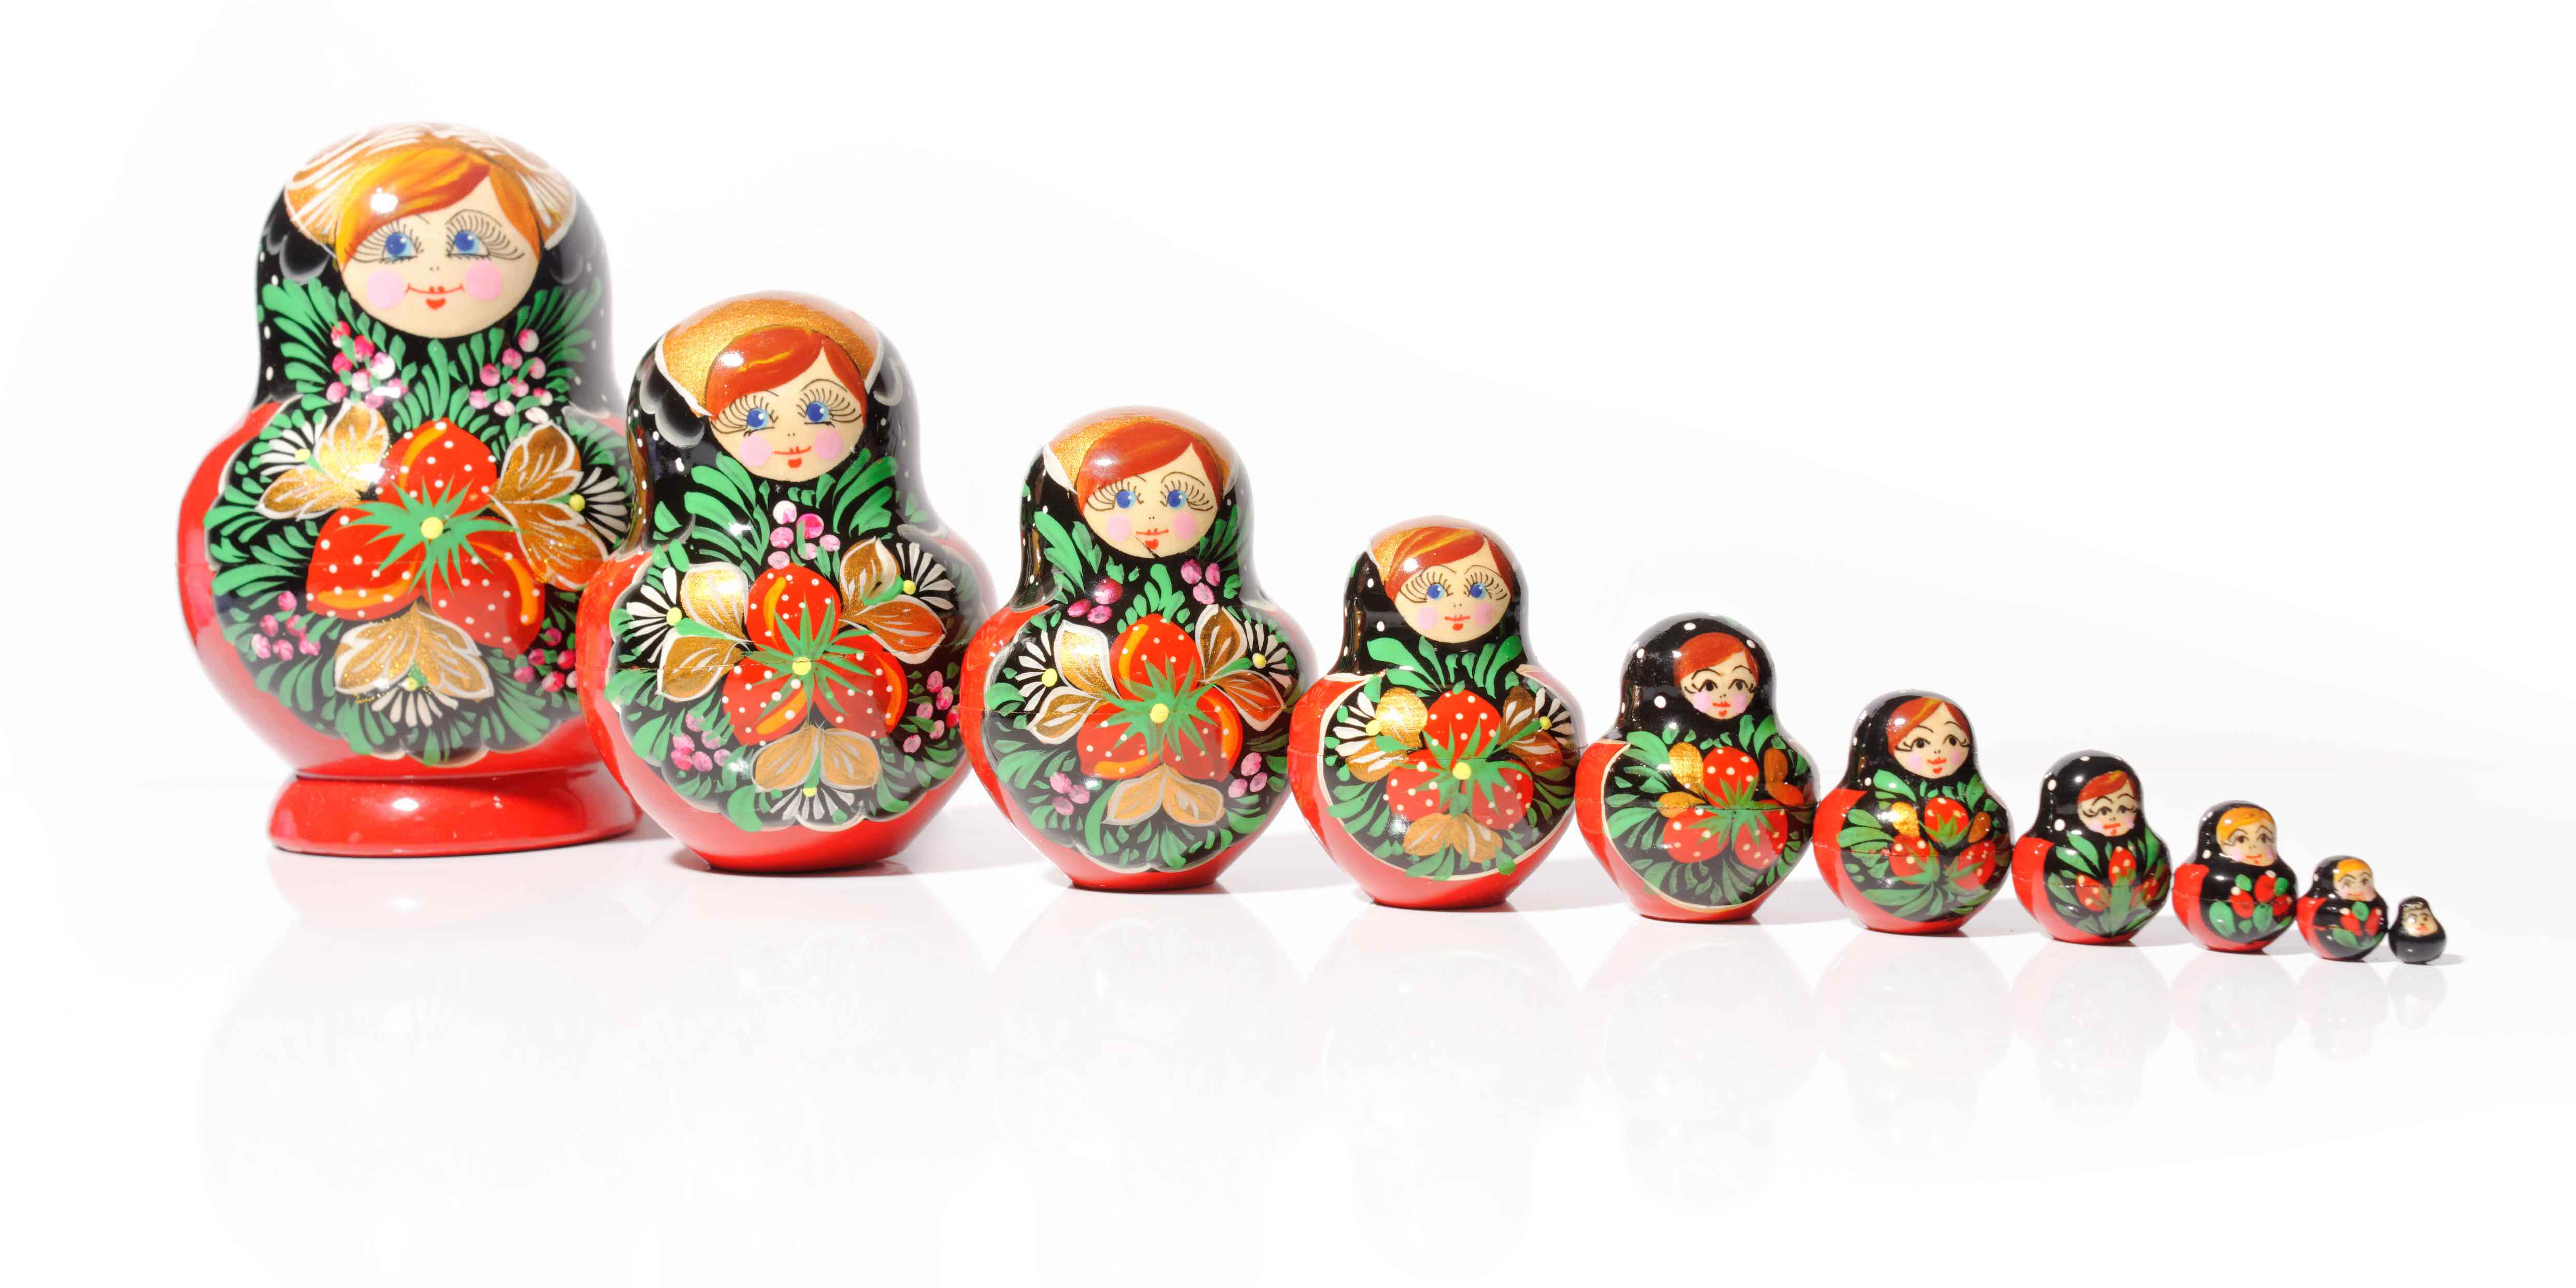
\includegraphics[width=\textwidth]{matr.jpg}
	\caption[Matryoshka doll]{Matryoshka doll\footnotemark, also called Russian doll. It consists of multiple wodden pieces that can be nested in each other.}
	\label{fig:matryoshka}
\end{figure}

\footnotetext{Copyright: S. Faric, \url{https://www.flickr.com/photos/tromal/6901848291/}, \href{https://creativecommons.org/licenses/by/2.0/}{CC BY 2.0 License}}

Before explaining the concept, we will elaborate what modularity is and why it is desirable. Then, we will go into more detail about the Smalltalk programming language and explain what modularity means in the context of Squeak/Smalltalk.

\section{Modularity}
\label{sec:meyermod}
What is \emph{modularity}? According to Myers, ``modularity is the single attribute of software that allows a program to be intellectually managable''~\cite{myers1978composite}. This thesis describes a module system for the Squeak programming language, i.e., a system that should help the programmer in writing modular code. According to Meyer, there are five requirements that a method or system should satisfy to be ``worthy of being called \emph{modular}''~\cite{Meyer:1988:OSC:534929}.

\paragraph{Decomposability}
If a design method supports modular decomposability, it helps the programmer in breaking down big components into smaller one. These subcomponents should be less complex, serve a different purpose, and be mostly independent of each other. Meyer compares decomposability with \emph{division of labor}: every subcomponent does a smaller, in itself less complex part of the job. Decomposability also benefits independent development of subcomponents, if these are mostly independent of each other. An example of a method supporting decomposability is top-down design.

\paragraph{Composability}
If a design method supports modular composability, it helps the programmer in building more complex components out of smaller ones. This encourages code reuse; subcomponents do not have to be implemented a second time. An example of composability are libraries. They fulfill a certain purpose, but cannot work on their own. Instead, they were designed to be used in another program, building complex functionality based on smaller pieces.

\paragraph{Understandability}
If a design method supports understandability, it helps programmers getting an overview and a broad understanding of an application more quickly. This goes hand in hand with decomposability: every subcomponent should be less complex and, therefore, easier to understand than the composed component. This is important to keep software maintainable and makes software development more time-efficient, as it reduces development time, because the programmer has to spend less time understanding the system.

\paragraph{Continuity}
If a design method supports continuity, it is easier to make changes to the program, since a single change should ideally only affect a single or at least a small number of modules. Every change should be confined to a very small number of modules. This is can be a side effect of decomposability, if done properly~\cite{Parnas:1972:CUD:361598.361623}. Continuity also makes it easier to extend the behavior of a program.

\paragraph{Protection}
If a design method supports protection, it helps the programmer writing code where program malfunctions are confined to a single or a small number of modules, instead of spreading across the entire program. For example, every subcomponent should have a well-specified interface and could check input parameters before running the actual implementation.

\section{The Squeak Programming Language}
\label{sec:intro_squeak_prog}
Smalltalk is a dynamically-typed, object-oriented, class-based programming language and Squeak\footnote{\url{http://squeak.org}}~\cite{Ingalls:1997:BFS:263698.263754} is a Smalltalk-80 dialect. It was originally developed by Alan Kay, Dan Ingalls, and Adele Goldberg. Dan Ingalls described Smalltalk-80 as a project whose purpose it is to ``provide computer support for the creative spirit in everyone.'' In his article \emph{Design Principles Behind Smalltalk}~\cite{Inga81a}, which appeared in August 1981 in the BYTE Magazine, he mentions some of the most fundamental principles behind the Smalltalk project. Some of these go hand in hand with modularity and can be further supported by a good module system.

\begin{itemize}
	\item ``Personal Mastery: If a system is to serve the creative spirit, it must be entirely comprehensible to a single individual.'' A module system can support understandability of a system by breaking up big components into smaller ones (\emph{hierarchical decomposition}) and hiding irrelevant implementation details.
	\item ``Factoring: Each independent component in a system would appear in only one place.'' A module system can encourage code reuse by making it easy to share behavior and reuse it in other modules, eliminating code duplication. %store shared behavior and components in a designated place that allows other components to take advantage of it and eliminate code duplication.
	\item ``Modularity: No component in a complex system should depend on the internal details of another component.'' Through information hiding, a module system can encourage programmers not to rely on implementation-specific behavior. A notion of what is considered a public interface can help keeping modules exchangable and increases understandability, since only the public interface should be sufficient to understand what a module is doing.
	\item ``Good Design: A system should be built with a minimum set of unchangable parts; those parts should be as generic as possible.'' Consequently, if we are to create a module system for Smalltalk, that system should build on top of a single fundamental concept, and all features and use cases should evolve out of this concept in a natural way, without any special corner cases.
\end{itemize}

\section{Outline of this Thesis}
The remainder of this thesis is structured as follows. Section~\ref{sec:problem} gives an overview of modular programming in Squeak/Smalltalk, shows what is possible already, and describes concrete points where we see room for improvement. Section~\ref{sec:concept} describes the concept of our module system in an abstract way, without diving into notation or implementation details. Section~\ref{sec:impl} describes the implementation of our module system in Squeak/Smalltalk, as well as corner cases and pitfalls. Section~\ref{sec:usecases} describes concrete use cases and provides examples, implemented in our module system, based on the shortcomings motivated in Section~\ref{sec:problem}. Sections~\ref{sec:related} and~\ref{sec:future} compare our implementation with other existing systems, and give an overview of the next steps, respectively. Finally, we give a short summary of our concept and implementation in Section~\ref{sec:summary}.

% \input{context}
% \input{solution}
% \chapter{Implementation}

\section{Meta Model and Instantiation}
Our system has a simple meta model for describing (nested) classes and their methods. The graphical user interface operates exclusively on the meta model and makes changes to it. The meta model can then be instantiated to generate the actual classes. When changes to the meta model are made, these changes can also be applied to already existing instantiations of the model, allowing giving programmers the feeling of working with a live system.

\paragraph{Smalltalk-80 Class/Meta Model}
Squeak already comes with a meta model: objects are instances of a classes, consequently, classes are also instances of a class. In Smalltalk, every class is an instance of its own meta class, which is in turn instance of \texttt{Metaclass}.

Our system allows class generation at runtime: class generator methods generate classes along with their respective meta classes. Therefore, we need a specification/blueprint that describes how a class generator method should construct a class. At first glance, it might seem logical to use meta classes; after all, a meta class is the class of a regular (non-meta) class and classes are instance generators. However, meta classes cannot be used as class object generators in a way required by our system for two reasons.

Firstly, meta classes do not have any information about their non-meta class counterpart: for example, they do not know anything about their instance methods or their instance variables. Instantiating a meta class would not generate a functional class object, which is why Smalltalk prohibits generating new instances of a meta class. In fact, the class \texttt{ClassBuilder} is used to create new classes and it always creates class objects alongs with their meta class objects.

Secondly, our system supports defining methods on the instance side and on the class side. Consequently, we do not only need to generate class object but also meta class objects. All meta classes are an instance of \texttt{Metaclass}. But if we wanted to generate different meta classes, we would need a different \texttt{Metaclass} class, each of which generates its corresponding meta class. In some programming languages, the instance-of chain carries on infinitely; Ruby is an example. However, in Smalltalk, every meta class is an instance of \texttt{Metaclass} and this is where the instance-of chain recurses: \texttt{Metaclass} is an instance of \texttt{Metaclass class}, which is an instance of \texttt{Metaclass}.

For this reason, we cannot use the Smalltalk-80 meta model to generate new classes on the fly and use our own simple meta model instead.

\paragraph{Nested Classes Meta Model}
Figure~\ref{fig:impl_meta_model} shows the meta model in our system. The meta model is built around specifications: there are specifications for classes, meta classes, and methods. A specification describes how its corresponding object is built. \texttt{ClassSpecification}s generate classes, \texttt{MetaclassSpecification}s generate meta classes, and \texttt{MethodSpecification}s generate methods. Since classes cannot exist without their respective meta classes, a class specification is always linked with its meta class specification and vice-versa. When a class specification is instantiated, the system generates both the class and the meta class. Meta class specifications cannot be instantiated.

\begin{figure}
	\centering
	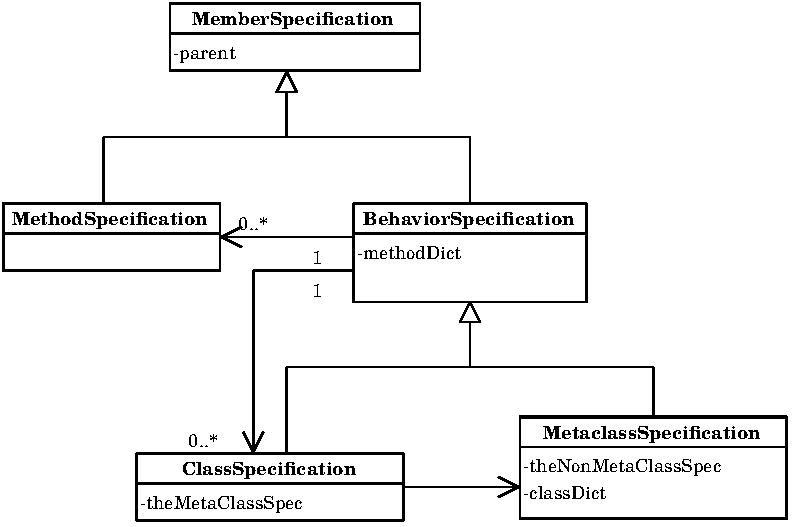
\includegraphics[scale=1]{metamodel.pdf}
	\caption{Meta Model for Nested Classes}
	\label{fig:impl_meta_model}
\end{figure}

\paragraph{Class Specifications}
A class specification describes classes. It has a collection of \texttt{MethodSpecification}s, representing instance methods of the class. Upon instantiation, all method specifications are instantiated within the target class. For every class specification, there is a corresponding method specification containing the source code of the class generator method in the parent's method dictionary. This method specification determines (when executed in the running system) to which class the methods will be added (\emph{target class}). Top-level classes are an exception: they are always a new subclass of the class \texttt{Module}.

\paragraph{Meta Class Specification}
A meta class specification describes meta classes. It has a collection of \texttt{MethodSpecification}s, representing class methods of the class (i.e., instance methods of the meta class). Upon instantiation, all method specifications are instantiated within the targer class' meta class. Consequently, meta classes do not method specifications associated with.

However, meta classes can have nested classes of their own. For every class defined in a meta class, there is a corresponding method specification present in the method dictionary (see previous paragraph).

\paragraph{Method Specification}
A method specification describes methods. It contains the source code of the method and stores information necessary for class caching and UI metadata. Whenever a method specification is instantiated, the method source code is compiled in the target class. 

Note, that different byte code must be generated for different target classes: for example, instance variable reads and write are compiled to parameterized\footnote{There are separate bytecodes for reading the first or second instance variable etc.} \texttt{pushRcvr:} and \texttt{popIntoRcvr:} bytecodes, where instance variables are referenced with their index\footnote{The first instance variable has index 0, second index variable has index 1, etc.}. In addition, the \texttt{outer} and the \texttt{enclosing} keyword must be bound to different method literals, depending on the lexical scope of the class.

\paragraph{Class Initialization}
Figure~\ref{fig:lazy_class_gen} illustrates how the system generates and initializes a nested class (class specification instantiation).

\begin{figure}
	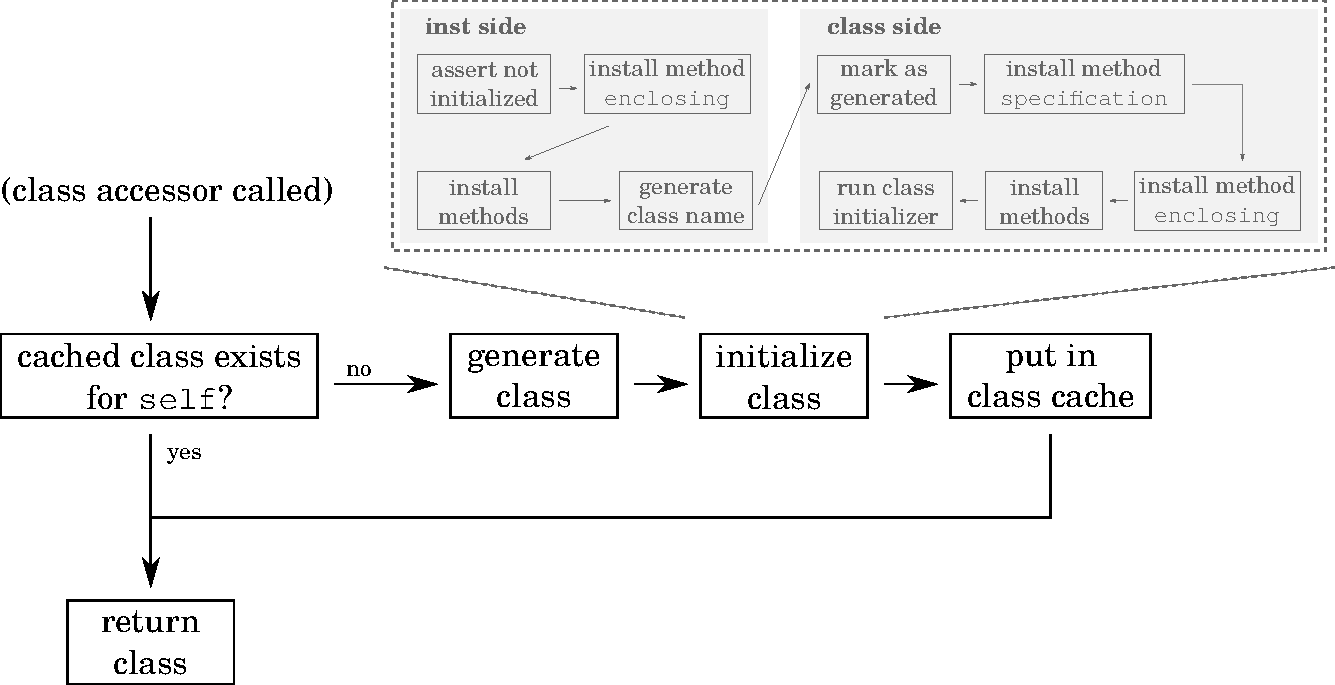
\includegraphics[width=\textwidth]{lazy_class_gen.pdf}
	\centering
	\caption{Lazy class generation and initialization}
	\label{fig:lazy_class_gen}
\end{figure}

Whenever a class accessor method is invoked, the method first checks if the class is already cached. If that is the case, it is returned. Otherwise, the class generator method called, returning an empty uninitialized class, i.e., all instance methods are still missing and only the superclass and the instance and class variables are set up correctly. The following list gives an overview of the steps necessary for initializing a class.

\begin{enumerate}
	\item Install \texttt{enclosing} instance method. This method returns the enclosing class.
	\item Install/compile all instance methods listed in the class specification.
	\item Generate the class name. The class name is a concatenation of the enclosing class' name and the selector of this class' accessor method. It is stored as an instance variable at \texttt{Class}. Note, that every class object is an instance of its meta class, which is a subclass of \texttt{Class}.
	\item Add a marker method to the meta class to mark it as generated. This makes is easy to check if a class is an ordinary (legacy) Smalltalk class or was generated within our system.
	\item Install \texttt{specification} class method. This method returns the class specification, which is useful for meta programming purposes.
	\item Install \texttt{enclosing} class method. This method is identical to the instance method.
	\item Install/compile all class methods listed in the meta class specification.
	\item Send \texttt{initialize} to the class object.
\end{enumerate}

Note, that class initialization is lazy. A class is only generated and initialized if the corresponding accessor method was called. All references to classes in the source code actually call the accessor method, making sure that the class is available when it is needed. 

Class generator methods can return subclasses of other classes; the superclass is referenced by calling the accessor method. Compared to the default package-loading process in Squeak, this makes class creation easier. In Squeak, the system has to analyze which classes are subclasses of each other, in order to create classes in the correct order (superclass has to exist before subclass is created). In our system, classes are created when their accessor method is called, and if these classes depend on another superclass, that superclass is created when the class generator method calls its accessor method (if it does not already exist).

\paragraph{Class Accessor Methods and Class Generator Methods}
For a nested class, two methods are installed on the meta class object: a class generator method, returning the class to which methods should be added (usually a newly-created subclass), and a class accessor method, checking whether the class was already created and is in the cache or calling the class generator method, otherwise.

The selector for the class accessor method is the name of the class. The selector for the class generator method is the same selector, but with a dollar sign prefix. This ensures that the method can only be called by using meta programming from our system, and also avoids accidential name clashes with other methods. For example, if a class is named \texttt{Foo}, the class accessor method has the selector \texttt{Foo} and the class generator method has the selector \texttt{\$Foo}.

\section{Anonymous Classes and Subclass Generation}
In Smalltalk, new classes are created by subclassing an already existing class. Squeak has special class, the \texttt{ClassBuilder}, containing all the functionality for creating the class object, the meta class object, giving the class a name, possibly migrating the old class and its instances (if an existing class was changed), and registering it in the \texttt{globals} dictionary.

Our system reuses the class builder and adds functionality for creating anonymous subclasses. Anonymous subclasses do not have a name and certain checks are omitted (e.g., if the class name starts with a capital letter). Also, anonymous subclasses are not added to the \texttt{globals} dictionary.

\paragraph{Subclass Notation}
Figure~\ref{fig:impl_subclass_squeak} shows how subclasses are created in Squeak. The first statement is a message send to \texttt{Object} which not only creates the subclass but also adds it to the \texttt{globals} dictionary. The second statement is also executable code that adds an instance variable to the meta class object. The difference between class variables and class instance variables is that class variables are shared among all subclasses, whereas class instance variables have different values for every class object~\cite{classvar1,classvar2}. For example, if \texttt{A} has a class variable \texttt{Bar} and \texttt{B} is a subclass of \texttt{A}, then both \texttt{A} and \texttt{B} share one variable \texttt{Bar}.

\begin{figure}[!htp]
\begin{lstlisting}
Object subclass: #NewClass
    instanceVariableNames: 'foo bar'
    classVariableNames: 'Bar'
    poolDictionaries: ''
    category: 'Demo-Experiments'.

NewClass class
	instanceVariableNames: 'Foo'.
\end{lstlisting}
\caption{Subclass notation in Squeak}
\label{fig:impl_subclass_squeak}
\end{figure}

Figure~\ref{fig:impl_subclass_nested} shows how subclassesa created in our system. \texttt{NewClass} is a class generator method and also the name of the new class. Therefore, it is no longer necessary to pass a symbol with the name of the new class to the \texttt{subclass:} method. Note, that the \textttt{<class>} pragma is necessary to distinguish between class generator methods and regular methods, which might accidentially return a class. Only in the former case, a class specification object is created.

\begin{figure}[!htp]
\begin{lstlisting}
NewClass
    < class >
    ^ Object 
    	subclassWithInstVars: 'foo bar'
    	classVars: 'Bar'
        classInstVars: 'Foo'
\end{lstlisting}
\caption{Subclass notation with nested classes}
\label{fig:impl_subclass_nested}
\end{figure}


\section{\texttt{thisOuter} and \texttt{thisScope}}

\section{Class Updates}
using instances weak array on specification

\section{Integration in Squeak}

\subsection{Module Repository}
replacement for Smalltalk dict

\subsection{IDE Support}
works in workspace, test runner. How to write tests? New system browser

\subsection{Debugger}
shows slightly different code (thisContext automatically inserted, generator methods)
% \input{evaluation}
% \chapter{Related Work}

\section{Class Name Clashes}

\subsection{Namespaces/Packages}
VisualWorks, Java, Ruby, Python

\subsection{Squeak Environments}

\subsection{Newspeak Modules}


\section{Dependency Management}

\subsection{Java Class Loader}

\subsection{Separate Compilation}

\subsection{External Configuration in Newspeak}


\section{Readability and Understandability}

\subsection{Smalltalk Packages}

\subsection{Hierarchical Decomposition}
Java, Python, Ruby, Newspeak, \ldots

\subsection{Information Hiding with Interfaces}


\section{Code Reuse}

\subsection{Multiple Inheritance}

\subsection{Mixins}
Ruby Modules, Python Multiple Inheritance, Newspeak, Jigsaw

\subsection{Traits}
Squeak implementation

% \input{conclusion}
%

% beispiel.

\chapter{Introduction}
This thesis describes the concept, the implementation, and concrete use cases of \emph{\msname}, a module system for and written in Squeak/Smalltalk. \msname used to be a popular Russian name and is believed to be the origin of the name \emph{Matryoshka}~\cite{dixon1998encyclopedia}, also known as Russian doll. Matryoshka dolls are wodden dolls that can be nested in each other (Figure~\ref{fig:matryoshka}), and are a metaphor for class nesting, the most fundamental concept of \msname.

\begin{figure}[!htp]
	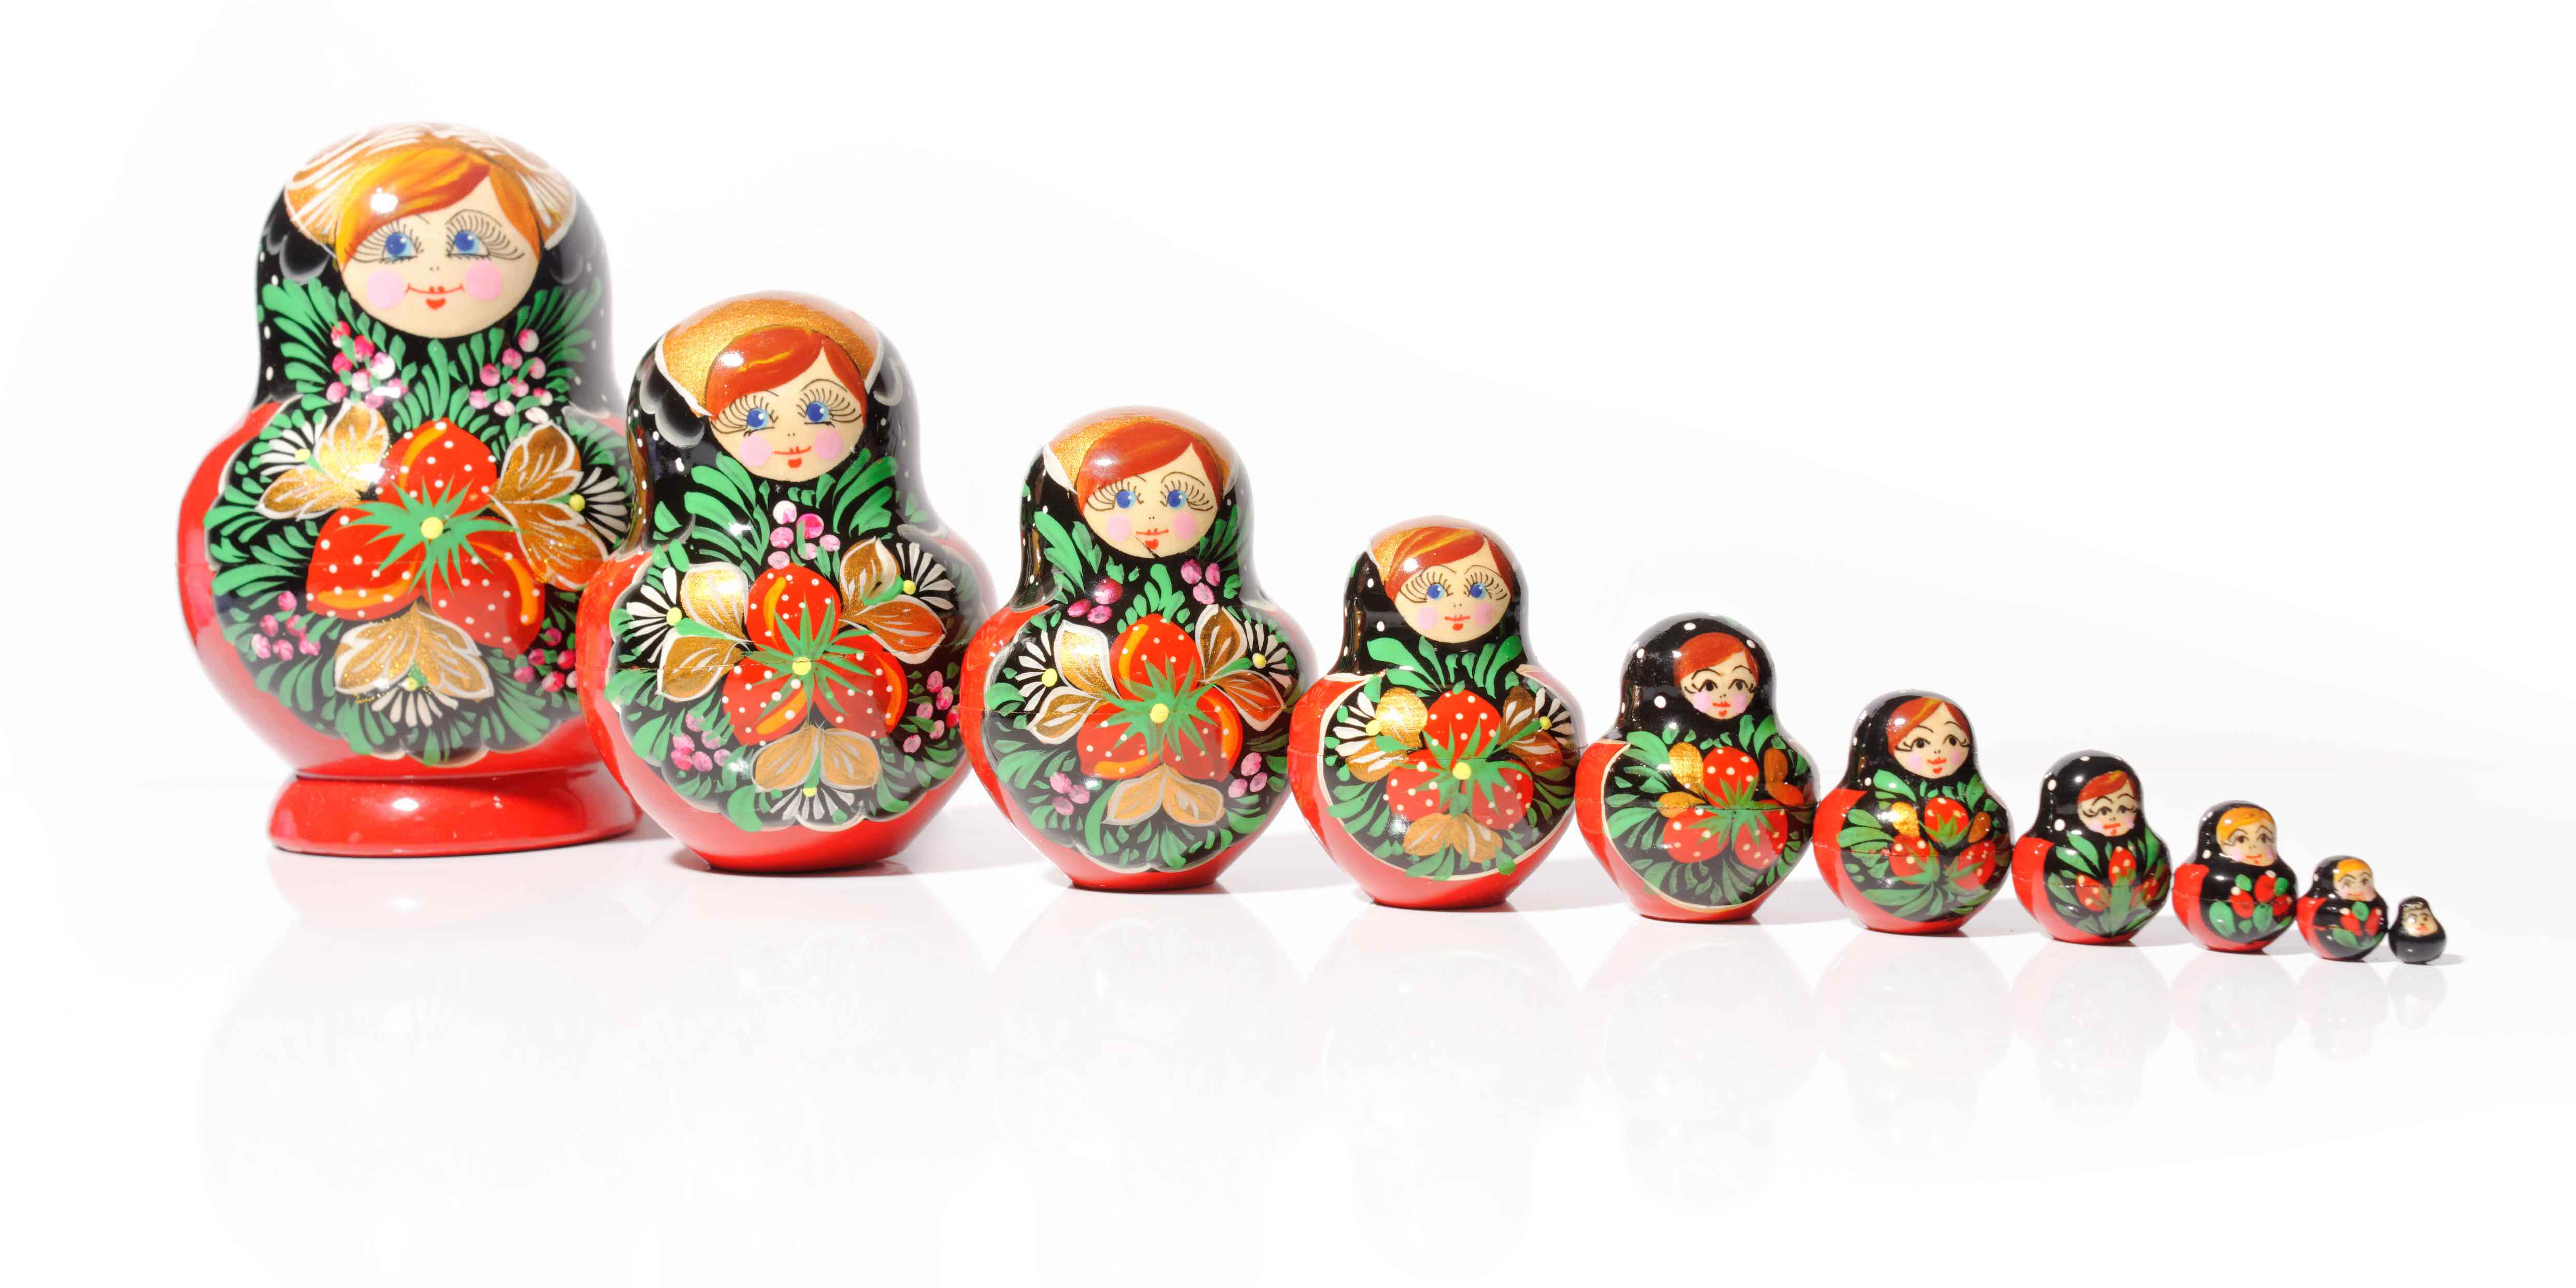
\includegraphics[width=\textwidth]{matr.jpg}
	\caption[Matryoshka doll]{Matryoshka doll\footnotemark, also called Russian doll. It consists of multiple wodden pieces that can be nested in each other.}
	\label{fig:matryoshka}
\end{figure}

\footnotetext{Copyright: S. Faric, \url{https://www.flickr.com/photos/tromal/6901848291/}, \href{https://creativecommons.org/licenses/by/2.0/}{CC BY 2.0 License}}

Before explaining the concept, we will elaborate what modularity is and why it is desirable. Then, we will go into more detail about the Smalltalk programming language and explain what modularity means in the context of Squeak/Smalltalk.

\section{Modularity}
\label{sec:meyermod}
What is \emph{modularity}? According to Myers, ``modularity is the single attribute of software that allows a program to be intellectually managable''~\cite{myers1978composite}. This thesis describes a module system for the Squeak programming language, i.e., a system that should help the programmer in writing modular code. According to Meyer, there are five requirements that a method or system should satisfy to be ``worthy of being called \emph{modular}''~\cite{Meyer:1988:OSC:534929}.

\paragraph{Decomposability}
If a design method supports modular decomposability, it helps the programmer in breaking down big components into smaller one. These subcomponents should be less complex, serve a different purpose, and be mostly independent of each other. Meyer compares decomposability with \emph{division of labor}: every subcomponent does a smaller, in itself less complex part of the job. Decomposability also benefits independent development of subcomponents, if these are mostly independent of each other. An example of a method supporting decomposability is top-down design.

\paragraph{Composability}
If a design method supports modular composability, it helps the programmer in building more complex components out of smaller ones. This encourages code reuse; subcomponents do not have to be implemented a second time. An example of composability are libraries. They fulfill a certain purpose, but cannot work on their own. Instead, they were designed to be used in another program, building complex functionality based on smaller pieces.

\paragraph{Understandability}
If a design method supports understandability, it helps programmers getting an overview and a broad understanding of an application more quickly. This goes hand in hand with decomposability: every subcomponent should be less complex and, therefore, easier to understand than the composed component. This is important to keep software maintainable and makes software development more time-efficient, as it reduces development time, because the programmer has to spend less time understanding the system.

\paragraph{Continuity}
If a design method supports continuity, it is easier to make changes to the program, since a single change should ideally only affect a single or at least a small number of modules. Every change should be confined to a very small number of modules. This is can be a side effect of decomposability, if done properly~\cite{Parnas:1972:CUD:361598.361623}. Continuity also makes it easier to extend the behavior of a program.

\paragraph{Protection}
If a design method supports protection, it helps the programmer writing code where program malfunctions are confined to a single or a small number of modules, instead of spreading across the entire program. For example, every subcomponent should have a well-specified interface and could check input parameters before running the actual implementation.

\section{The Squeak Programming Language}
\label{sec:intro_squeak_prog}
Smalltalk is a dynamically-typed, object-oriented, class-based programming language and Squeak\footnote{\url{http://squeak.org}}~\cite{Ingalls:1997:BFS:263698.263754} is a Smalltalk-80 dialect. It was originally developed by Alan Kay, Dan Ingalls, and Adele Goldberg. Dan Ingalls described Smalltalk-80 as a project whose purpose it is to ``provide computer support for the creative spirit in everyone.'' In his article \emph{Design Principles Behind Smalltalk}~\cite{Inga81a}, which appeared in August 1981 in the BYTE Magazine, he mentions some of the most fundamental principles behind the Smalltalk project. Some of these go hand in hand with modularity and can be further supported by a good module system.

\begin{itemize}
	\item ``Personal Mastery: If a system is to serve the creative spirit, it must be entirely comprehensible to a single individual.'' A module system can support understandability of a system by breaking up big components into smaller ones (\emph{hierarchical decomposition}) and hiding irrelevant implementation details.
	\item ``Factoring: Each independent component in a system would appear in only one place.'' A module system can encourage code reuse by making it easy to share behavior and reuse it in other modules, eliminating code duplication. %store shared behavior and components in a designated place that allows other components to take advantage of it and eliminate code duplication.
	\item ``Modularity: No component in a complex system should depend on the internal details of another component.'' Through information hiding, a module system can encourage programmers not to rely on implementation-specific behavior. A notion of what is considered a public interface can help keeping modules exchangable and increases understandability, since only the public interface should be sufficient to understand what a module is doing.
	\item ``Good Design: A system should be built with a minimum set of unchangable parts; those parts should be as generic as possible.'' Consequently, if we are to create a module system for Smalltalk, that system should build on top of a single fundamental concept, and all features and use cases should evolve out of this concept in a natural way, without any special corner cases.
\end{itemize}

\section{Outline of this Thesis}
The remainder of this thesis is structured as follows. Section~\ref{sec:problem} gives an overview of modular programming in Squeak/Smalltalk, shows what is possible already, and describes concrete points where we see room for improvement. Section~\ref{sec:concept} describes the concept of our module system in an abstract way, without diving into notation or implementation details. Section~\ref{sec:impl} describes the implementation of our module system in Squeak/Smalltalk, as well as corner cases and pitfalls. Section~\ref{sec:usecases} describes concrete use cases and provides examples, implemented in our module system, based on the shortcomings motivated in Section~\ref{sec:problem}. Sections~\ref{sec:related} and~\ref{sec:future} compare our implementation with other existing systems, and give an overview of the next steps, respectively. Finally, we give a short summary of our concept and implementation in Section~\ref{sec:summary}.

\chapter{Modularity Problems in Squeak}
\label{sec:problem}
In this section, we describe and evaluate how Squeak can be used to write modular programs at the moment. Based on our observations and programming experience with Squeak, there are three areas in which we see room for improvement. For every area, we will describe what the problem is and how it is currently solved in Squeak.

\paragraph{Class-based Modularity}
In pure Smalltalk, classes are the highest level of modular units. Classes are first-class objects and can be passed around. This functionality can be used to make behavior interchangable and promotes loose coupling. Classes are Smalltalk's way of sharing behavior with a number of objects, i.e., it is a form of code reuse. Squeak also supports Traits, a design method for composing class of pieces of behavior (see Section~\ref{sec:rel_traits}).

Smalltalk is, as most object-oriented and class-based programming languages, amenable to well-established software design patterns~\cite{Gamma:1995:DPE:186897}, making it easier to write maintainable and understandable code.

\section{Duplicate Class Names}
In Squeak, there can only be only one class with a certain name. Whenever, the programmer tries to add another class with the same name, a conflict occurs. When source code is loaded into the system with the Monticello version control system, the system asks the programmer if the already existing class should be replaced. As a workaround, it is good practice to add unique namespace prefixes to all class names in an application. 

Squeak has packages~\cite{Nierstrasz:2009:SE:1816759}, but these are not used as namespaces. Their purpose is to make it easier to find existing classes (like method protocols). They are also used as deployment units. The programmer does usually not load single classes into the system. Instead, packages (groups of classes) are loaded. 

Squeak environments provide a way to have multiple classes with the same name in one image. However, they suffer from poor tool support and do not integrate well with some of the other goals (e.g., code reuse) for our system. See Section~\ref{sec:rel_sq_env} for a detailed discussion of Squeak environments and why we did not use them in this system.

\paragraph{Example}
\begin{figure}[!htp]
\dirtree{%
.1 \framebox{\textbf{BroBreakout}}.
.2 BroBall.
.2 BroBlock.
.2 BroBoundary.
.2 BroBreakout.
.2 BroExplosion.
.2 BroLevelBuilder.
.2 BroLevelStatistics.
.2 BroLevelStatisticsItem.
.2 BroLevelView.
.2 BroLevelWorld.
.2 BroMenuLabel.
.2 BroMenuView.
.2 \textit{BroPowerup}.
.2 BroPowerupAccelerate.
.2 BroPowerupBall.
.2 BroPowerupDecelerate.
.2 BroPowerupEnlarge.
.2 BroPowerupShrink.
.2 BroRacket.
.2 \textit{BroView}.
.2 BroWelcomeView.
}
\caption[Breakout class structure]{Breakout class structure. All classes have the \texttt{Bro} namespace prefix and are contained in the package \texttt{BroBreakout}.}
\label{fig:conc_breakout}
\end{figure}

Consider the game Breakout (Figure~\ref{fig:conc_breakout}, see also Section~\ref{sec:usecase_hierach_decomp}). This application uses \texttt{Bro} as a prefix for all classes. If we would not use namespace prefixes, generic class names like \texttt{Block} or \texttt{Ball} would be likely to collide with other classes. On the other hand, if all application and library developers adhere to this convention, it is unlikely that class name classes occur.

\section{Dependency Managment}
Dependency management describes the task of keeping track of dependencies and ensuring that required dependencies are available to the application in question. We destinguish between two cases of dependency management: internal dependency management, i.e., the application specifies all dependencies, and external dependency managment (\emph{external configuration}), i.e., user of the application specifies all dependencies. But before managing dependencies, we need a versioning concept that allows us to represent library versions in an image.

\paragraph{Versioning}
There are situations when it is useful to have multiple versions of the same library in one image; for example, if there are two different applications installed and both require the same library, but in different versions. Old versions of a library might have bugs that an application has to work around. The application might then not work with a newer library, where the bug is fixed. Furthermore, the public API of a library might change with new versions, especially if it is a new major version.

Therefore, we need a versioning mechanism in \msname, that helps us to store and reference different versions of the same application or library in one image. Part of this mechanism must be a way to develop new library versions, and a mechanism to reference a certain version.

\paragraph{Internal Dependency Management}
In this case, every application or library specifies itself which dependencies (and their versions) it depends on. The application effectively maintains the list of dependencies itself. Consequently, the application is coupled to its dependencies and cannot be used with different versions or implementations without changing its source code.

\paragraph{External Configuration}
In this case, the dependency management is delegated to the client of an application or library. What the application specifies is that it requires some dependency implementing a certain interface, but not what exact dependency it is exactly or in what version. This mechanism is also called \emph{dependency injection} and used heavily in the Java world~\cite{Prasanna:2009:DI:1795686}. Dependency injection is also known as \emph{inversion of control}~\cite{fowlerioc}, because it inverts the control of dependencies: it is shifted from the application or library in question to the user/client. External configuration is beneficial for modularity, because it supports loose coupling of application and dependencies. This, in turn, promotes understandability, maintainablity, and exchangability (code reuse), because an application cannot rely on implementation details of a loosely bound dependency.

\paragraph{Dependency Management in Squeak}
In Squeak, there can currently only be one version of a library or application installed at a time. Monticello is used a source code management system and can be used to load new versions of the source code into an image. Metacello is a package management system (see Section~\ref{sec:rel_metacello}), similar to Maven in Java. Every Metacello package has a configuration class containing a list of external dependencies and internal packages to load for every version, along with the location of an external repository where the packages should be loaded from~\cite{metacellodraft}.

External configuration can simulated in Smalltalk by writing class constructors that accept other dependencies as parameters. These dependencies should then be stored in instance variables and only be accessed using instance variables. However, this technique has two pitfalls. Firstly, dependencies have to be forwarded to all other classes, resulting in boilerplate code. Secondly, only instance methods can benefit from external configuration, because class methods are shared among instances (configurations) of the class.

\section{Hierarchical Decomposition}
Smalltalk packages allow the programmer to group together what belongs together~\cite{Eckel:2002:TJ:579108}. This is especially useful in big projects with many classes and allows for a form of modular decomposition. Different criterias for modular decomposition have been proposed: e.g., functional decompositon (making every step in the \emph{flowchart} a module) or information hiding~\cite{Parnas:1972:CUD:361598.361623}. The following list shows some benefits of good modular decomposition.

\begin{itemize}
	\item Changability (continuity): only few classes are affected when changing a detail.
	\item Independent development: classes can be developed in parallel.
	\item Understandability: in order to understand the behavior of a class, it is sufficient to read code within that class.
\end{itemize}

What we want to achieve is hierarchical decomposition~\cite{Blume:1999:HM:325478.325518}, which is in a basic form realized in Java packages, Ruby namespace module, or Python modules. It can increase comprehensibility of the overall system when it acts as some kind of decision tree that helps the programmer finding a submodule corresponding to a certain functionality in an unknown application. 

It also allows for fine-grained dependency management: for example, it is considered good practice in many programming languages to keep import statements as small as possible. Import statements also act as documentation, giving the reader of the source code a rough idea of what the source code might do. Furthermore, if a functionality is nested in a submodule, it is likely that it is written in a more general way, such that it might be reused elsewhere in the application without bigger changes.

If the source code is functionally decomposed in a hierarchical way~\cite{Tsui:2009:ESE:1823101}, it is also easier to understand single submodules of the system. The reader of the source code might only be interested in a certain level of detail (e.g., no low-level functionality), and then skip deeply nested submodules~\cite{hierarch1} (information hiding or abstraction). Since in functional decomposition, the purpose of nested modules is usually only to serve their enclosing modules, readers can start off with a high-level idea of the module is doing by going through the first few levels of nesting, and dive in deeper as needed.

Therefore, one of the requirements for our system is to provide a mechanism for hierarchical code decomposition that is more than just one level deep (Smalltalk packages).

\paragraph{Example}
Consider the game SpaceCleanup, which is a simple bomberman clone (Figure~\ref{fig:prob_space_cleanup_org}, see also Section~\ref{sec:usecase_hierach_decomp}). The source code for this game is organized in multiple packages. For example, all items in the game are grouped in the package \texttt{SpaceCleanup-Items}. Besides this obvious single-level decomposition, the game is actually already functionally decomposed in a hierarchical way. For example, \texttt{ScuLevel} represents a level in the game. A level consists of multiple tiles (\texttt{ScuTile}). A tile cannot exist without a level; its sole purpose is to serve \texttt{ScuLevel}. Similarly, items always belong to a tile and cannot be used without a tile. All in all, SpaceCleanup is already functionally decomposed, but this decomposition is not fully reflected in the class organization.

\begin{figure}[!htp]
\dirtree{%
.1 \framebox{\textbf{SpaceCleanup-Core}}.
.2 ScuEventDispatcher.
.2 ScuGame.
.2 ScuGameBuildState.
.2 ScuGameConfigState.
.2 ScuGameOverState.
.2 ScuGamePausedState.
.2 ScuGameRunningState.
.2 \textit{ScuGameState}.
.2 ScuGameWonState.
.2 \textit{ScuMonsterStrategy}.
.2 ScuMonsterRandomStrategy.
.2 ScuMonsterToPlayerStrategy.
}
\vspace{10pt}
\dirtree{%
.1 \framebox{\textbf{SpaceCleanup-Items}}.
.2 ScuBucket.
.2 \textit{ScuDestructibleItem}.
.2 ScuFloor.
.2 \textit{ScuItem}.
.2 ScuMonster.
.2 \textit{ScuMovingItem}.
.2 ScuPickUpItem.
.2 ScuPlayer.
.2 ScuPortal.
.2 ScuSlime.
.2 ScuWall.
.2 ScuWater.
}
\vspace{10pt}
\dirtree{%
.1 \framebox{\textbf{SpaceCleanup-Level}}.
.2 ScuLevel.
.2 \textit{ScuLevelBuilder}.
.2 ScuGridPatternLevelBuilder.
.2 ScuRandomLevelBuilder.
.2 ScuTile.
}
\vspace{10pt}
\dirtree{%
.1 \framebox{\textbf{SpaceCleanup-Resources}}.
.2 ScuResourceManager.
}
\vspace{10pt}
\dirtree{%
.1 \framebox{\textbf{SpaceCleanup-UI}}.
.2 ScuCheatWindow.
.2 ScuConfigurationWindow.
.2 ScuControls.
.2 ScuGameInformation.
}
\caption[SpaceCleanup class organization]{SpaceCleanup class organization. All classes have the \texttt{Scu} namespace prefix and are grouped in five packages, according to their responsibilities.}
\label{fig:prob_space_cleanup_org}
\end{figure}


%\section{Code Reuse}
%share behavior among multiple classes

\chapter{Nested Class Modularity in Squeak}
\label{sec:concept}
In this chapter, we describe the main concept of this work: classes as class members. Similar concepts are part of programming languages like Java, Ruby, Python, and Newspeak. Our concept follows closely the Newspeak notion of nested classes, but without making invasive changes to the Smalltalk programming language or the underlying virtual machine.

\section{Nested Classes}
In Smalltalk, every object is an instance of a class, defining the object's instance variables and the messages it understands. Consequently, a class is also an instance of its so-called meta class. Every meta class is an instance of \texttt{Metaclass} (Figure~\ref{fig:impl_squeak_meta}). In the remainder of this work, we denote the meta class of a class \texttt{C} by \texttt{C class}. Every Smalltalk image has a \texttt{globals} dictionary\footnote{Squeak also supports \emph{environments}, effectively making it possible to compile methods in the context of another \texttt{globals} dictionary. See Section~\ref{sec:rel_sq_env} for more details.}, mapping symbols to class objects (or other objects), so that references to classes can be resolved at compile time. This implies that all references to classes are early bound.

\msname extends the Smalltalk class organization as follows: in addition to regular methods, we introduce the concept of \emph{class generator methods}. Such a method generates a class and is associated with a set $I$ of instance methods and a set $C$ of class methods. Whenever the method is invoked, the system first executes the method body, then adds $I$ to the resulting class and $C$ to the resulting meta class, and finally returns the resulting class. For performance reasons, \msname also caches the result, meaning that a class is only generated once\footnote{Parameterized classes are an exception.}.

\paragraph{Details}
Class generator methods are only allowed as class-side methods. Class generators as instance-side methods seem to provide neglectable benefits and make the implementation of our system more complicated. We discuss instance-side class generator methods in more detail in the Section~\ref{sec:future_inst_side}.

A class generated by a class generator method is anonymous: it is not listed in the \texttt{globals} dictionary and can only be referenced using message sends to its enclosing class\footnote{It can also be referenced by sending the \texttt{class} message to one of its instances}. Consequently, its name is a concatenation of all class names on the path from the top-level class to the class in question.


\paragraph{Notation and Example}
\begin{wrapfigure}{l}{0.5\textwidth}
	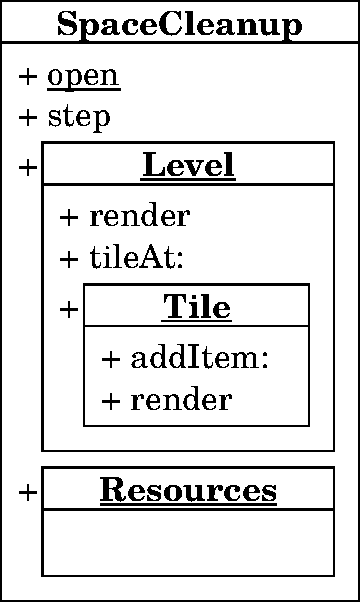
\includegraphics[scale=0.75]{nested_notation.pdf}
	\centering
	\caption[Example: Nested classes]{Example: nested classes. A class can have class-side member classes.}
	\label{fig:concept_nested_notation}
\end{wrapfigure}

Figure~\ref{fig:concept_nested_notation} shows an example of nested classes in \msname. \texttt{SpaceCleanup} is a top-level class, i.e., it is part of the \texttt{globals} dictionary and known everywhere in the system; it can be referenced by just writing the identifier \texttt{SpaceCleanup}. It has one instance method \texttt{step} and two class methods \texttt{open} and \texttt{Level}. In accordance with UML notation, class-side method selectors are underlined. 

\texttt{SpaceCleanup class>>Level} is a class generator method that is associated with a set of instance methods $\{\mbox{\texttt{render}, \texttt{tileAt:}}\}$ and a set of class methods $\{\mbox{\texttt{Tile}}\}$. The name of the class it generates is \texttt{SpaceCleanup Level}, which is in that case also a valid Smalltalk code expression that evaluates to the generated class. \texttt{SpaceCleanup class>>Level class>>Tile} is a class generator method that generates \texttt{SpaceCleanup Level Tile}. Note, that we use the \texttt{>>} notation to not only reference methods but also the classes they generate, in case they are class generator methods.

Top-level classes are called \emph{modules}. All other classes are called \emph{nested classes}. The class in which another class is nested is called the \emph{enclosing class}.

%\begin{figure}[!htp]
%	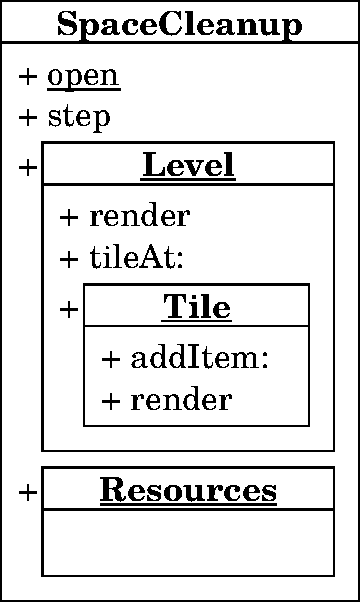
\includegraphics[scale=0.5]{nested_notation.pdf}
%	\centering
%	\caption{Nested Classes Example}
%	\label{fig:concept_nested_notation}
%\end{figure}

\section{Accessing the Lexical Scope}
Within a method, it might be necessary to access the lexical scope, in order to send messages to enclosing classes. For example, a method might want to reference a class defined in an enclosing class (e.g., \texttt{SpaceCleanup Resources} in \texttt{SpaceCleanup class>>Level class>>Tile>>render}). For this reason, \msname introduces new keywords, in addition to \texttt{self} and \texttt{super}, which are already present in every Smalltalk dialect. This is a point where we extended the programming language. Figure~\ref{fig:concept_keywords} gives an overview of all method lookup-related keywords in the system.

\begin{figure}[!htp]
	\centering
	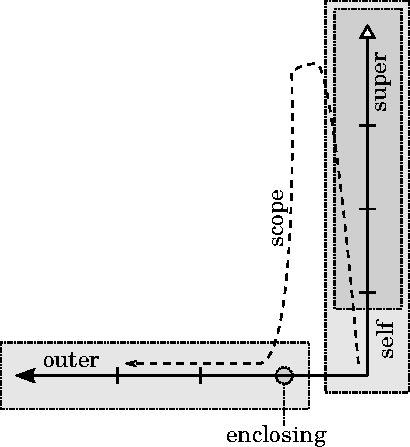
\includegraphics[scale=1]{lookup_keywords.pdf}
	\caption[Keywords for superclass and lexical scope access]{Keywords for superclass and lexical scope access. The lookup starts at \texttt{self}, and continues with the lexical scope.}
	\label{fig:concept_keywords}
\end{figure}

\subsection{\texttt{self} Keyword}
This keyword is used make a message send within an object. The receiver is the same object as the sender and the lookup starts at the (polymorphic) class of the receiver. If that class does not provide a corresponding method, the lookup continues in the superclass hierarchy. If no class in the superclass hierarchy has a corresponding method, a \texttt{MethodNotUnderstood} error is raised.

\begin{wrapfigure}{l}{0.5\textwidth}
	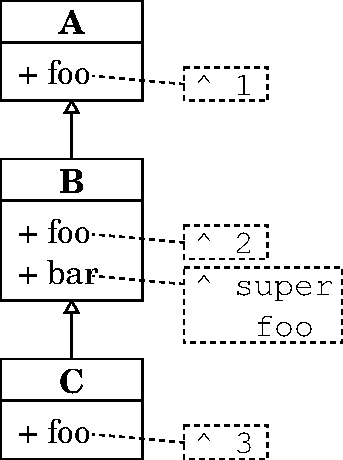
\includegraphics[scale=0.75]{super_binding.pdf}
	\centering
	\caption[Example: Binding of \texttt{super}]{Example: Binding of \texttt{super}. The method lookup starts at the superclass of the calling method's class.}
	\label{fig:concept_super_binding}
\end{wrapfigure}

\subsection{\texttt{super} Keyword}
This keyword is also used to make a message send within an object. Again, the receiver is the same object as the sender, but the lookup starts at the superclass of the sender's method class. Note, that \texttt{super} is bound to the superclass of the method class, not the superclass of the receiver's class. For example, in Figure~\ref{fig:concept_super_binding}, \texttt{Monster new defaultImage} returns \texttt{Resources errorPic}, because, in \texttt{MovingItem>>defaultImage}, \texttt{super} is bound to \texttt{Item}, even though the receiver \texttt{Monster new} is an instance of \texttt{Monster}.

\subsection{\texttt{enclosing} Keyword}
This keyword is an implementation artifact. It can be used for meta programming purposes, but should be avoided in general. It is used to make a message send to the class that contains the current class. Consider, for example, that we want to send a message \texttt{levelBackground} to class \texttt{SpaceCleanup Resources} within \texttt{SpaceCleanup class>>Level>>render} in Figure~\ref{fig:concept_nested_notation}. Either one of the following two statements works in this case\footnote{The enclosing class of an object that is not a class is its class' enclosing class.}.

\begin{itemize}
	\item \texttt{SpaceCleanup Resources levelBackground.}
	\item \texttt{enclosing Resources levelBackground.}
\end{itemize}

\texttt{enclosing} is a keyword that evaluates to the method owner's enclosing class upon method compilation. Note, that \texttt{enclosing} is bound to the method's lexical scope, not the receiver class' lexical scope.

Figure~\ref{fig:concept_lexical_thisouter} illustrates how \texttt{enclosing} is bound. In \texttt{SpaceCleanup class>>Item class>>player}, \texttt{enclosing} is bound to \texttt{SpaceCleanup}. In contrast, \texttt{UberSpaceClean\-up class>>Item class>>evilMonster} binds \texttt{enclosing} to \texttt{UberSpaceCleanup}. Consequently, \texttt{SpaceCleanup Item monster} calls \texttt{SpaceCleanup Resources monster} and so does \texttt{UberSpaceCleanup Item monster}, even though the receiver of \texttt{monster} is \texttt{UberSpaceCleanup Item} and not \texttt{SpaceCleanup Item} in the latter case. Note, that \texttt{UberSpaceCleanup Item evilMonster} calls the method in \texttt{UberSpaceCleanup Resources}, because \texttt{evilMonster}'s lexically enclosing class is \texttt{UberSpaceCleanup}.

\begin{figure}[!htp]
	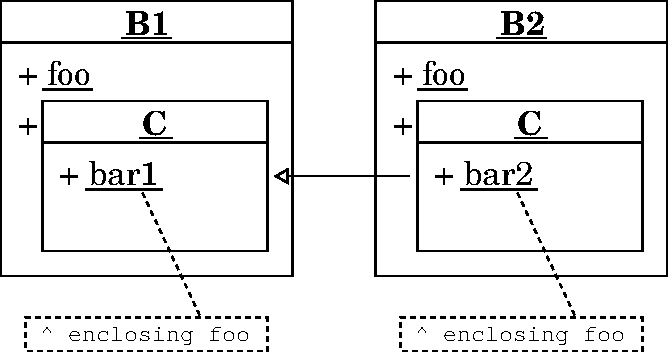
\includegraphics[scale=0.75]{nested_lexical1.pdf}
	\centering
	\caption[Example: Binding of \texttt{enclosing}]{Example: Binding of \texttt{enclosing}. The keyword is bound to enclosing class of the class where the method containing the keyword is contained.}
	\label{fig:concept_lexical_thisouter}
\end{figure}

Note, that \texttt{enclosing} can be used for meta programming purposes; however, it should be avoided in general, because it can lead to fragile code that makes too many assumptions about the structure of the class nesting. A later refactoring could then lead to broken code. Probably for the same reason, Smalltalk does not have a \texttt{super} keyword that does the lookup only in the superclass\footnote{However, there is a method \texttt{Class>>superclass}.} (single-level super). \msname provides a \texttt{scope} keyword that should be used instead.

\subsection{\texttt{enclosing} Method}
In addition to \texttt{enclosing}, every class in the system has a method \texttt{enclosing} that returns the enclosing class (\emph{owner}) of the receiver, making it possible to send messages to enclosing classes which are more than one level away. If, for example, in Figure~\ref{fig:concept_nested_notation}, \texttt{SpaceCleanup class>>Level class>>Tile>>render} wants to send the message \texttt{tileBackground} to \texttt{SpaceCleanup Resources}, either one of the following two statements works.

\begin{itemize}
	\item \texttt{SpaceCleanup Resources tileBackground.}
	\item \texttt{enclosing enclosing Resources tileBackground.}
\end{itemize}

Again, the method \texttt{enclosing} should be avoided in general, but is useful to implement parts of our system with code written in the system itself and for meta programming purposes. The statement \texttt{enclosing enclosing} would be somewhat similar to a \texttt{super super} statement. Arguably, this can result in verbose and complicated code, and is at the very least questionable with regards to the law of demeter. Note, that, in contrast to the \texttt{outer} keyword, the message send of \texttt{enclosing} to \texttt{enclosing} is no longer bound to the lexical scope of the method.

\subsection{\texttt{outer} Keyword}
\label{sec:concept_outer}
This keyword is used to make a message send to classes in the lexical scope. Whenever a message is sent to \texttt{outer}, the message is first interpreted as a send to \texttt{enclosing}. If that message send fails, the message is sent to the second-level enclosing class in the current lexical scope. Eventually, the message is sent to a top-level class, if no other class understands the message. If even that message send is not understood, the selector is looked up in the \texttt{globals} dictionary. If the selector is absent, a \texttt{MessageNotUnderstood} error is raised.

\texttt{outer} is similar to \texttt{super}, with the difference that \texttt{outer} does a horizontal lookup (lexical scope) and \texttt{super} does a vertical lookup (superclass chain). Note, that messages sent to \texttt{outer} are sent to an object different from \texttt{self}.

\paragraph{Example}
Figure~\ref{fig:concept_outer_1} illustrates how message sends to \texttt{outer} are looked up. Consider, for example, that the method \texttt{foo} in \texttt{A1 B C} calls \texttt{outer bar}. Both \texttt{A1 B C foo} and \texttt{A2 B C foo} call \texttt{A1 class>>bar} in this case, because \texttt{outer} is bound to the lexical scope of the method.

Figure~\ref{fig:concept_outer_2} shows why it is important that \texttt{outer} is bound to the lexical scope. In this example, \texttt{D B2} is a subclass of \texttt{A B1}. If the \texttt{outer} lookup simply traversed the chain of enclosing classes of the (late bound) receiver class, i.e., first lookup in \texttt{self enclosing}, then \texttt{self enclosing enclosing}, etc., the message send of \texttt{bar} would fail in \texttt{D B2 C foo}. As another consequence, a nested class might then no longer be able to access a class defined in an enclosing class if the nested class is subclassed and nested in a different enclosing class, since classes are accessed using message sends.

\begin{figure}[!htp]
\begin{subfigure}[b]{\textwidth}
	\centering
	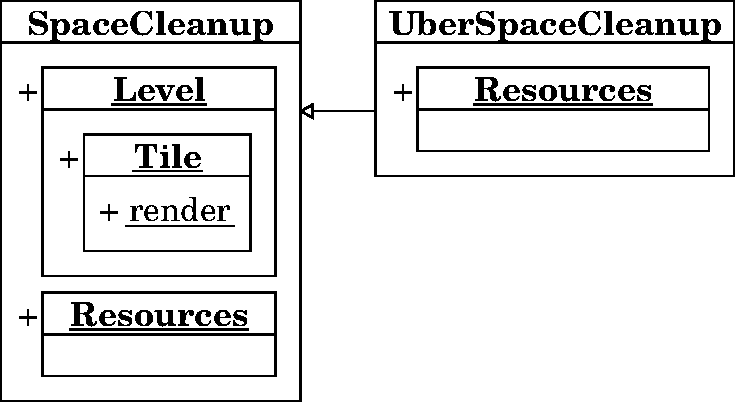
\includegraphics[scale=0.75]{outer_keyword.pdf}
	\caption{Subclassed top-level class}
	\label{fig:concept_outer_1}
\end{subfigure}

\vspace{15pt}

\begin{subfigure}[b]{\textwidth}
	\centering
	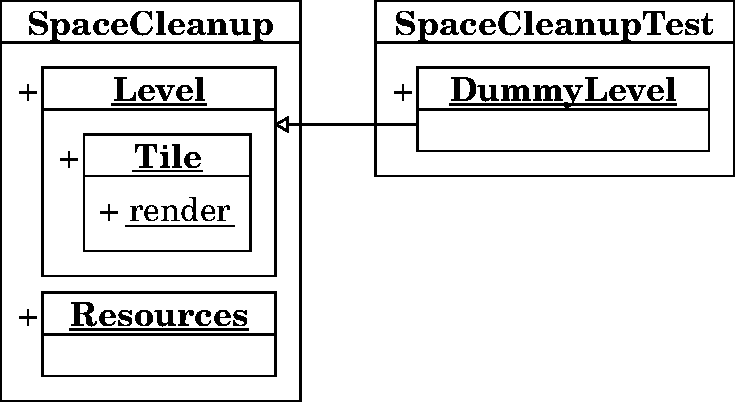
\includegraphics[scale=0.75]{outer_keyword_2.pdf}
	\caption{Subclassed nested class with different enclosing class}
	\label{fig:concept_outer_2}
\end{subfigure}

\caption[Example: \texttt{outer} keyword]{Example: \texttt{outer} keyword. Message sends to \texttt{outer} are looked up with respect to the lexical scope of the method, instead of following the chain of enclosing classes (owner hierarchy).}
\end{figure}

%The method \texttt{enclosing} can be used to traverse the the lexical scope of a class. Arbitrarily many \texttt{enclosing} sends can be chained, as long as the respective receiver still has an enclosing class and is, therefore, not a top-level class. Arguably, this can result in verbose and complicated code, and is at the very least questionable with regards to the law of demeter.

%In addition to \texttt{enclosing}, \msname provides the \texttt{outer} keyword, bound to the method's lexical scope. 

% If that message send fails, the message is sent to \texttt{enclosing enclosing}, and, eventually, to the top-level class, if no other class in the lexical scope understands the message. 

\subsection{\texttt{scope} Keyword}
This keyword combines \texttt{super} and \texttt{outer}: a message sent to \texttt{scope} is first treated as a \texttt{self} send. If the message is not understood, it is treated as an \texttt{outer} send.

\msname essentially first looks up the methods in \texttt{self}, then in the superclass hierarchy, and then in the lexical scope. This is how the method lookup in Java works, also known as \emph{comb semantics}~\cite{bracha2007interaction}. Newspeak uses a different lookup: it first looks for a method in the receiver's class, then in the lexical scope, and finally in superclass hierarchy~\cite{bracha:modules_as_objects}.

%The statement \texttt{enclosing enclosing m1} in the previous example can also be written as \texttt{scope m1}. If the method \texttt{m1} would now be moved to its enclosing class (if it had one), the lookup would still succeed. However, \texttt{scope} exposes the risk of accidentially capturing method names in superclasses or the lexical chain.

\subsection{Implicit \texttt{scope} Receiver}
In \msname, references to globals are in fact message sends with \texttt{scope} as implicit receiver. This should make it easier for Smalltalk programmers to write code in \msname, even if they do not know about \texttt{enclosing} and \texttt{scope}. It also makes the code less verbose and easier to read.

Whenever code references an identifier that is not a temporary variable, not an instance variable, and not a \emph{special} object/keyword\footnote{\texttt{self}, \texttt{super}, \texttt{thisContext}, \texttt{scope}, \texttt{outer}, \texttt{enclosing}}, the compiler replaces that identifier with a message send to \texttt{scope}.

Consider, for example, that we want to reference class \texttt{A B} within \texttt{A class>>B class>>C>>bar} in Figure~\ref{fig:concept_nested_notation}. Either one of the following two statements works in this case.

\begin{itemize}
	\item \texttt{A B.}
	\item \texttt{enclosing.}
	\item \texttt{enclosing enclosing B.}
	\item \texttt{outer B.}
	\item \texttt{scope B.}
	\item \texttt{B.}
\end{itemize}

In this example, we used the implicit \texttt{scope} receiver for class lookup, which is in our opinion the most useful case. However, any unary method in \texttt{self}, the lexical scope, or the superclass hierarchy can in fact be looked up this way. One can argue that this is bad practice and should be forbidden for methods that are not class generator methods. However, it is allowed in Newspeak and other programming languages like Java, and seems to work well. Note, that only unary messages can have an implicit \texttt{scope} receiver, since we would have to change the Smalltalk syntax, otherwise.

\section{Parameterized Classes}
In \msname, classes are accessed using message sends. Since messages can have parameters, it seems natural to have parameterized class accessor methods, and, therefore, parameterized classes. All examples shown in the previous sections use unparameterized classes, i.e., class generator methods are always unary. Class generator methods can, however, also have binary selectors or selectors with a higher arity. For memory conservation reasons, these classes are then no longer cached.

\begin{wrapfigure}{l}{0.5\textwidth}
	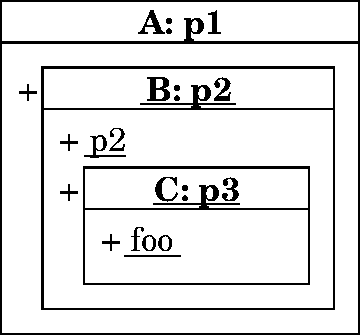
\includegraphics[scale=0.75]{nested_notation_params.pdf}
	\centering
	\caption[Example: Parameterized classes]{Example: Parameterized classes. A class can have parameters accessible with message sends to \texttt{enclosing}.}
	\label{fig:concept_param_classes}
\end{wrapfigure}

Parameterized classes can be used to make modules externally configurable or to implement mixins. We will present some conrete use cases in Section~\ref{sec:usecases}.

The arguments passed to a parameterized class generator method are considered when a message is sent to \texttt{enclosing}. At first, the system tries to send the message to the enclosing class. If that fails, \msname checks if the selector corresponds to one of the parameter names in the enclosing class' class generator method.

Consider, for example, that method \texttt{A: class>>B: class>>C: class>>foo} in Figure~\ref{fig:concept_param_classes} contains the following statements.
\begin{itemize}
	\item \texttt{scope p3}: method lookup succeeds in \texttt{A: class>>B: class>>C:} and returns the class parameter \texttt{p3}.
	\item \texttt{scope p2}: method lookup succeeds in \texttt{A: class>>B:} and calls the method \texttt{p2}, which shadows the class parameter \texttt{p2}.
	\item \texttt{scope p1}: method lookup succeeds in \texttt{A:} and returns the class parameter \texttt{p1}.
\end{itemize}

\section{Inheriting Nested Classes}
\label{sec:concept_inh_nested_cl}
Nested classes are accessed using methods returning the generated class. They are similar to class instance variables in a sense that nested classes belong to the enclosing class object. Therefore, a subclass of the enclosing class has its own nested class, i.e., the nested classes might have the same methods and variables declared, but they are different objects. Nested classes can be overridden in subclasses of enclosing classes, just as regular methods can be overridden. The following paragraphs give an overview of how a subclass of an enclosing class can customize the nested class.

\paragraph{Override with Nested Class}
A subclass of an enclosing class can define a new nested class. The programmer simply adds a new class generator method with the same selector to the subclass. The superclass will keep using the old nested class, whereas the subclass will use the new one, because the method lookup ends in the subclass when the corresponding class accessor method is found. The new nested class will only have the methods defined for the subclass' nested class and not inherit or copy any methods from the superclass' nested class.

\paragraph{Override with Regular Method}
A subclass of an enclosing class can replace (override) a nested class with a regular method. The programmer simply adds a new method which is not a class generator method to the subclass.

\paragraph{Extend Inherited Nested Class without Subclassing}
A subclass can extend the inherited nested class, i.e., the nested class in the subclass will have the same superclass as the nested class in the superclass. However, the nested class in the subclass will have all methods defined for the nested class in the superclass and additionally all methods defined for the nested class in the subclass. Duplicate methods will be replaced, similarly to extension methods in Squeak.

\begin{figure}[!htp]
\begin{subfigure}[b]{\textwidth}
	\centering
	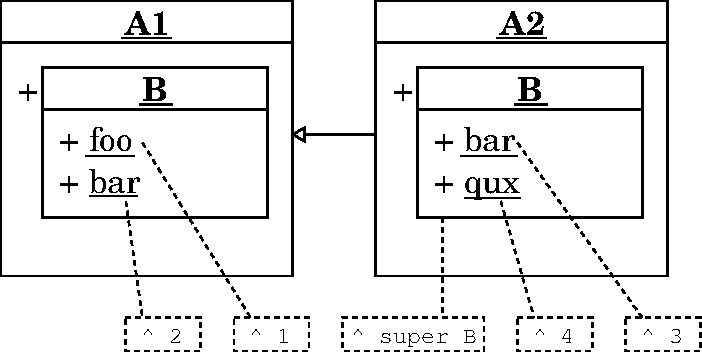
\includegraphics[scale=0.75]{nested_super_1.pdf}
	\caption{Extending inherited nested classing}
	\label{fig:impl:extend_inherited_class}
\end{subfigure}

\vspace{15pt}

\begin{subfigure}[b]{\textwidth}
	\centering
	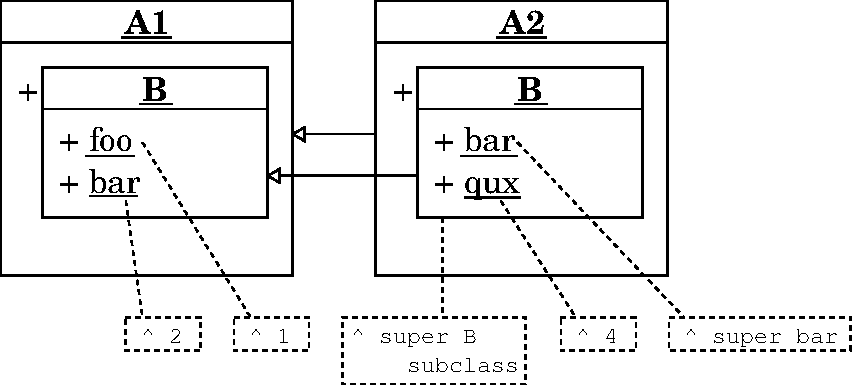
\includegraphics[scale=0.75]{nested_super_2.pdf}
	\caption{Subclassing inherited nested classing}
	\label{fig:impl:subclass_inherited_class}
\end{subfigure}

\caption[Example: Extending/subclassing nested classes]{Example: Extending and subclassing nested classes. Subclassing inherited nested classes leads to parallel class hierarchies.}
\end{figure}

Figure~\ref{fig:impl:extend_inherited_class} shows an example of a nested class extension. Class \texttt{A2} is a subclass of \texttt{A1}, which defines a nested class \texttt{B}. Therefore, both classes \texttt{A1} and \texttt{A2} have a nested class \texttt{B}. \texttt{A2} extends \texttt{B} by perfoming a super call. The following list gives an overview of how the classes \texttt{B} behave.

\begin{itemize}
	\item \texttt{A1 B foo}: returns 1.
	\item \texttt{A1 B bar}: returns 2.
	\item \texttt{A1 B qux}: raises \texttt{MessageNotUnderstood}, because \texttt{qux} is not defined on \texttt{A1 B}.
	\item \texttt{A2 B foo}: returns 1, because \texttt{A2 B} has all methods defined for \texttt{A1 B}.
	\item \texttt{A2 B bar}: returns 3, because that method was replaced in \texttt{A2 B}.
	\item \texttt{A2 B qux}: returns 4.
\end{itemize}

Note, that \texttt{A1 B} and \texttt{A2 B} have the same superclass, but are different class objects. \texttt{A2 B} is \emph{not} a subclass of \texttt{A1 B}. When \texttt{A2 B} is invoked for the first time, \msname first generates the class \texttt{A1 B} (because of the \texttt{super} call) and caches it for \texttt{A2 B}\footnote{Caches are receiver-specific.}. That class is then \emph{reinitialized} according to \texttt{A2 B} (without making a subclass), i.e., all methods defined for \texttt{A2 B} are added. A subsequent call to \texttt{A1 B} will not return the previous generated and extended class for \texttt{A2}, because the class cache works on a per-receiver basis.

Also note, that if we actually wanted to extend \texttt{A1 B} and alias it as \texttt{A2 B}, which is technically similar to an extension method in Smalltalk (see Section~\ref{sec:usecases_ext_meth}), then \texttt{A2 B} should be defined as \texttt{\^{} A1 B}, because the receiver of the message \texttt{B} will then be \texttt{A1} instead of \texttt{A2}. 

At the moment, there is no way to add additional instance variables or class variables to an extended nested class, because the class definition (containing the definition of variables) is done in the \texttt{super} call. 

\paragraph{Subclass Inherited Nested Class}
A subclass can subclass the inherited nested class, i.e., the nested class in the subclass is a subclass of the nested class in the superclass. Effectively, this results in a parallel class hierarchy. The nested subclass can override methods and use \texttt{super} to call methods in the nested superclass.

Figure~\ref{fig:impl:subclass_inherited_class} shows an example for subclassing a nested class, which is similar to Figure~\ref{fig:impl:extend_inherited_class}. Note, that \texttt{A2 B} is now a subclass of \texttt{A1 B} and \texttt{super} calls in \texttt{A2 B} now start their lookup in \texttt{A1 B}. The new subclass \texttt{A2 B} behaves like the class in the previous example, except for \texttt{A2 B bar}. That statement returns 2, because the \texttt{super} call invokes \texttt{A1 class>>B class>>foo}.


\chapter{Implementation}

\section{Meta Model and Instantiation}
Our system has a simple meta model for describing (nested) classes and their methods. The graphical user interface operates exclusively on the meta model and makes changes to it. The meta model can then be instantiated to generate the actual classes. When changes to the meta model are made, these changes can also be applied to already existing instantiations of the model, allowing giving programmers the feeling of working with a live system.

\paragraph{Smalltalk-80 Class/Meta Model}
Squeak already comes with a meta model: objects are instances of a classes, consequently, classes are also instances of a class. In Smalltalk, every class is an instance of its own meta class, which is in turn instance of \texttt{Metaclass}.

Our system allows class generation at runtime: class generator methods generate classes along with their respective meta classes. Therefore, we need a specification/blueprint that describes how a class generator method should construct a class. At first glance, it might seem logical to use meta classes; after all, a meta class is the class of a regular (non-meta) class and classes are instance generators. However, meta classes cannot be used as class object generators in a way required by our system for two reasons.

Firstly, meta classes do not have any information about their non-meta class counterpart: for example, they do not know anything about their instance methods or their instance variables. Instantiating a meta class would not generate a functional class object, which is why Smalltalk prohibits generating new instances of a meta class. In fact, the class \texttt{ClassBuilder} is used to create new classes and it always creates class objects alongs with their meta class objects.

Secondly, our system supports defining methods on the instance side and on the class side. Consequently, we do not only need to generate class object but also meta class objects. All meta classes are an instance of \texttt{Metaclass}. But if we wanted to generate different meta classes, we would need a different \texttt{Metaclass} class, each of which generates its corresponding meta class. In some programming languages, the instance-of chain carries on infinitely; Ruby is an example. However, in Smalltalk, every meta class is an instance of \texttt{Metaclass} and this is where the instance-of chain recurses: \texttt{Metaclass} is an instance of \texttt{Metaclass class}, which is an instance of \texttt{Metaclass}.

For this reason, we cannot use the Smalltalk-80 meta model to generate new classes on the fly and use our own simple meta model instead.

\paragraph{Nested Classes Meta Model}
Figure~\ref{fig:impl_meta_model} shows the meta model in our system. The meta model is built around specifications: there are specifications for classes, meta classes, and methods. A specification describes how its corresponding object is built. \texttt{ClassSpecification}s generate classes, \texttt{MetaclassSpecification}s generate meta classes, and \texttt{MethodSpecification}s generate methods. Since classes cannot exist without their respective meta classes, a class specification is always linked with its meta class specification and vice-versa. When a class specification is instantiated, the system generates both the class and the meta class. Meta class specifications cannot be instantiated.

\begin{figure}
	\centering
	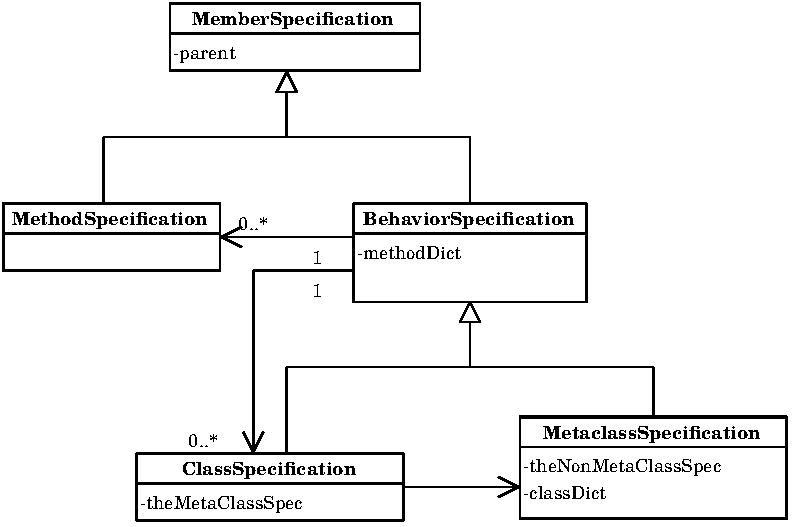
\includegraphics[scale=1]{metamodel.pdf}
	\caption{Meta Model for Nested Classes}
	\label{fig:impl_meta_model}
\end{figure}

\paragraph{Class Specifications}
A class specification describes classes. It has a collection of \texttt{MethodSpecification}s, representing instance methods of the class. Upon instantiation, all method specifications are instantiated within the target class. For every class specification, there is a corresponding method specification containing the source code of the class generator method in the parent's method dictionary. This method specification determines (when executed in the running system) to which class the methods will be added (\emph{target class}). Top-level classes are an exception: they are always a new subclass of the class \texttt{Module}.

\paragraph{Meta Class Specification}
A meta class specification describes meta classes. It has a collection of \texttt{MethodSpecification}s, representing class methods of the class (i.e., instance methods of the meta class). Upon instantiation, all method specifications are instantiated within the targer class' meta class. Consequently, meta classes do not method specifications associated with.

However, meta classes can have nested classes of their own. For every class defined in a meta class, there is a corresponding method specification present in the method dictionary (see previous paragraph).

\paragraph{Method Specification}
A method specification describes methods. It contains the source code of the method and stores information necessary for class caching and UI metadata. Whenever a method specification is instantiated, the method source code is compiled in the target class. 

Note, that different byte code must be generated for different target classes: for example, instance variable reads and write are compiled to parameterized\footnote{There are separate bytecodes for reading the first or second instance variable etc.} \texttt{pushRcvr:} and \texttt{popIntoRcvr:} bytecodes, where instance variables are referenced with their index\footnote{The first instance variable has index 0, second index variable has index 1, etc.}. In addition, the \texttt{outer} and the \texttt{enclosing} keyword must be bound to different method literals, depending on the lexical scope of the class.

\paragraph{Class Initialization}
Figure~\ref{fig:lazy_class_gen} illustrates how the system generates and initializes a nested class (class specification instantiation).

\begin{figure}
	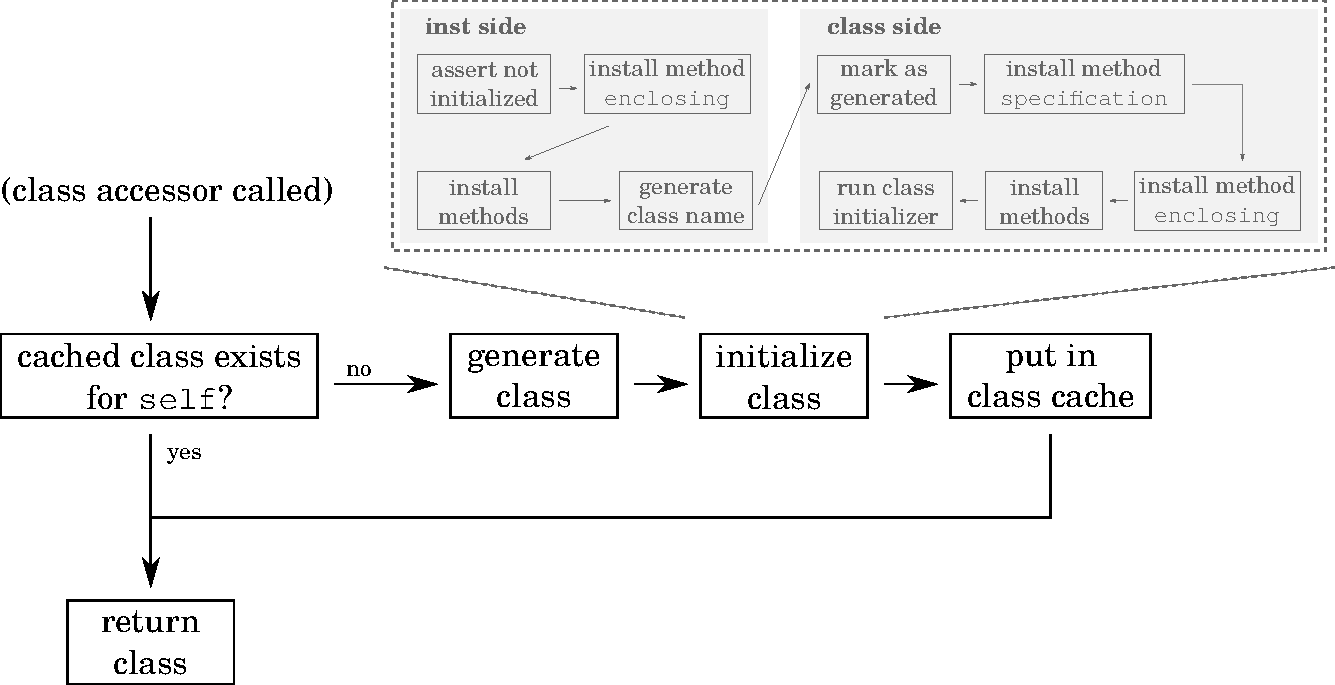
\includegraphics[width=\textwidth]{lazy_class_gen.pdf}
	\centering
	\caption{Lazy class generation and initialization}
	\label{fig:lazy_class_gen}
\end{figure}

Whenever a class accessor method is invoked, the method first checks if the class is already cached. If that is the case, it is returned. Otherwise, the class generator method called, returning an empty uninitialized class, i.e., all instance methods are still missing and only the superclass and the instance and class variables are set up correctly. The following list gives an overview of the steps necessary for initializing a class.

\begin{enumerate}
	\item Install \texttt{enclosing} instance method. This method returns the enclosing class.
	\item Install/compile all instance methods listed in the class specification.
	\item Generate the class name. The class name is a concatenation of the enclosing class' name and the selector of this class' accessor method. It is stored as an instance variable at \texttt{Class}. Note, that every class object is an instance of its meta class, which is a subclass of \texttt{Class}.
	\item Add a marker method to the meta class to mark it as generated. This makes is easy to check if a class is an ordinary (legacy) Smalltalk class or was generated within our system.
	\item Install \texttt{specification} class method. This method returns the class specification, which is useful for meta programming purposes.
	\item Install \texttt{enclosing} class method. This method is identical to the instance method.
	\item Install/compile all class methods listed in the meta class specification.
	\item Send \texttt{initialize} to the class object.
\end{enumerate}

Note, that class initialization is lazy. A class is only generated and initialized if the corresponding accessor method was called. All references to classes in the source code actually call the accessor method, making sure that the class is available when it is needed. 

Class generator methods can return subclasses of other classes; the superclass is referenced by calling the accessor method. Compared to the default package-loading process in Squeak, this makes class creation easier. In Squeak, the system has to analyze which classes are subclasses of each other, in order to create classes in the correct order (superclass has to exist before subclass is created). In our system, classes are created when their accessor method is called, and if these classes depend on another superclass, that superclass is created when the class generator method calls its accessor method (if it does not already exist).

\paragraph{Class Accessor Methods and Class Generator Methods}
For a nested class, two methods are installed on the meta class object: a class generator method, returning the class to which methods should be added (usually a newly-created subclass), and a class accessor method, checking whether the class was already created and is in the cache or calling the class generator method, otherwise.

The selector for the class accessor method is the name of the class. The selector for the class generator method is the same selector, but with a dollar sign prefix. This ensures that the method can only be called by using meta programming from our system, and also avoids accidential name clashes with other methods. For example, if a class is named \texttt{Foo}, the class accessor method has the selector \texttt{Foo} and the class generator method has the selector \texttt{\$Foo}.

\section{Anonymous Classes and Subclass Generation}
In Smalltalk, new classes are created by subclassing an already existing class. Squeak has special class, the \texttt{ClassBuilder}, containing all the functionality for creating the class object, the meta class object, giving the class a name, possibly migrating the old class and its instances (if an existing class was changed), and registering it in the \texttt{globals} dictionary.

Our system reuses the class builder and adds functionality for creating anonymous subclasses. Anonymous subclasses do not have a name and certain checks are omitted (e.g., if the class name starts with a capital letter). Also, anonymous subclasses are not added to the \texttt{globals} dictionary.

\paragraph{Subclass Notation}
Figure~\ref{fig:impl_subclass_squeak} shows how subclasses are created in Squeak. The first statement is a message send to \texttt{Object} which not only creates the subclass but also adds it to the \texttt{globals} dictionary. The second statement is also executable code that adds an instance variable to the meta class object. The difference between class variables and class instance variables is that class variables are shared among all subclasses, whereas class instance variables have different values for every class object~\cite{classvar1,classvar2}. For example, if \texttt{A} has a class variable \texttt{Bar} and \texttt{B} is a subclass of \texttt{A}, then both \texttt{A} and \texttt{B} share one variable \texttt{Bar}.

\begin{figure}[!htp]
\begin{lstlisting}
Object subclass: #NewClass
    instanceVariableNames: 'foo bar'
    classVariableNames: 'Bar'
    poolDictionaries: ''
    category: 'Demo-Experiments'.

NewClass class
	instanceVariableNames: 'Foo'.
\end{lstlisting}
\caption{Subclass notation in Squeak}
\label{fig:impl_subclass_squeak}
\end{figure}

Figure~\ref{fig:impl_subclass_nested} shows how subclassesa created in our system. \texttt{NewClass} is a class generator method and also the name of the new class. Therefore, it is no longer necessary to pass a symbol with the name of the new class to the \texttt{subclass:} method. Note, that the \textttt{<class>} pragma is necessary to distinguish between class generator methods and regular methods, which might accidentially return a class. Only in the former case, a class specification object is created.

\begin{figure}[!htp]
\begin{lstlisting}
NewClass
    < class >
    ^ Object 
    	subclassWithInstVars: 'foo bar'
    	classVars: 'Bar'
        classInstVars: 'Foo'
\end{lstlisting}
\caption{Subclass notation with nested classes}
\label{fig:impl_subclass_nested}
\end{figure}


\section{\texttt{thisOuter} and \texttt{thisScope}}

\section{Class Updates}
using instances weak array on specification

\section{Integration in Squeak}

\subsection{Module Repository}
replacement for Smalltalk dict

\subsection{IDE Support}
works in workspace, test runner. How to write tests? New system browser

\subsection{Debugger}
shows slightly different code (thisContext automatically inserted, generator methods)
\chapter{Use Cases}
\label{sec:usecases}

\section{Avoiding Class Name Clashes}
\begin{wrapfigure}{l}{0.55\textwidth}
	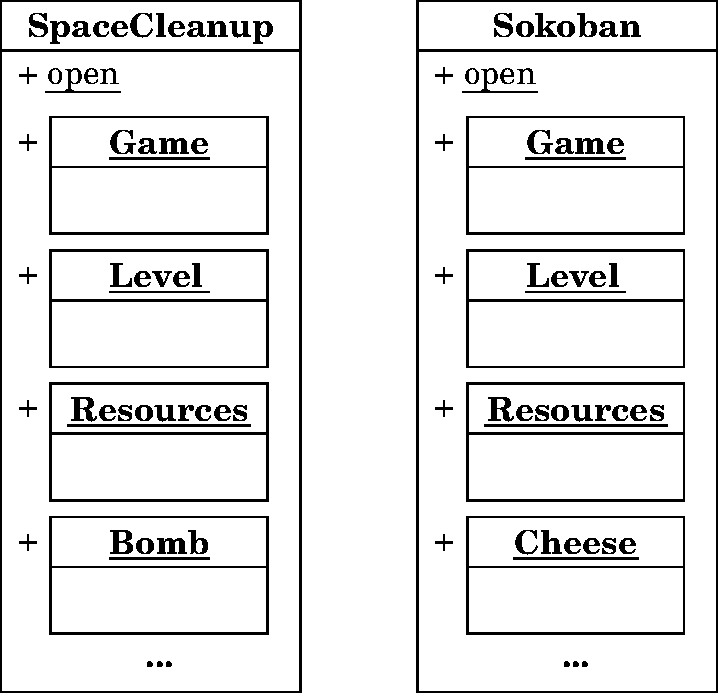
\includegraphics[width=0.5\textwidth]{usecase_class_clash.pdf}
	\centering
	\caption{Resolving class name clashes with class nesting}
	\label{fig:use_class_clash}
\end{wrapfigure}

In this example, class nesting is used to avoid class name clashes and to give every class a unique fully qualified name. Consider, that we want two load two computer games in a single Squeak image. The first game is a bomberman game, providing classes \texttt{Game}, \texttt{Level}, \texttt{Resources} among others. The second game is a Sokoban game, and has three classes with the same name. Without our system, this would be a problem: as soon as another class with the same is installed, the old one is overwritten with the new name.

With our system, two classes with the same name can coexist in the same image, as long as they are nested within different classes (Figure~\ref{fig:use_class_clash}).

Note, that, for example, \texttt{Bomberman Game} and \texttt{Sokoban Game} are different classes. Whenever a class inside \texttt{Bomberman} references \texttt{Game} using the source code statement \texttt{scope Game} or \texttt{Game} (equivalent statement), the method lookup recurses in the enclosing classes, until \texttt{Game} is found in the \texttt{Bomberman} class.

\section{Module Versioning and Dependency Management}
In this example, class nested is used to keep multiple different versions of the same library in one image. This is necessary if two applications require different versions of the same library. In the best case, the API of a library should not change within one major version, such that a newer library version should work with an application that was developed with an older library version. However, sometimes, application developers have to work around known bugs or rely on implementation-specific classes which are not designed to be used by library users and subject to change. In that case, application code can break when suddenly a different version of the library is used.

\subsection{Representing Module Versions}
\begin{wrapfigure}{l}{0.55\textwidth}
	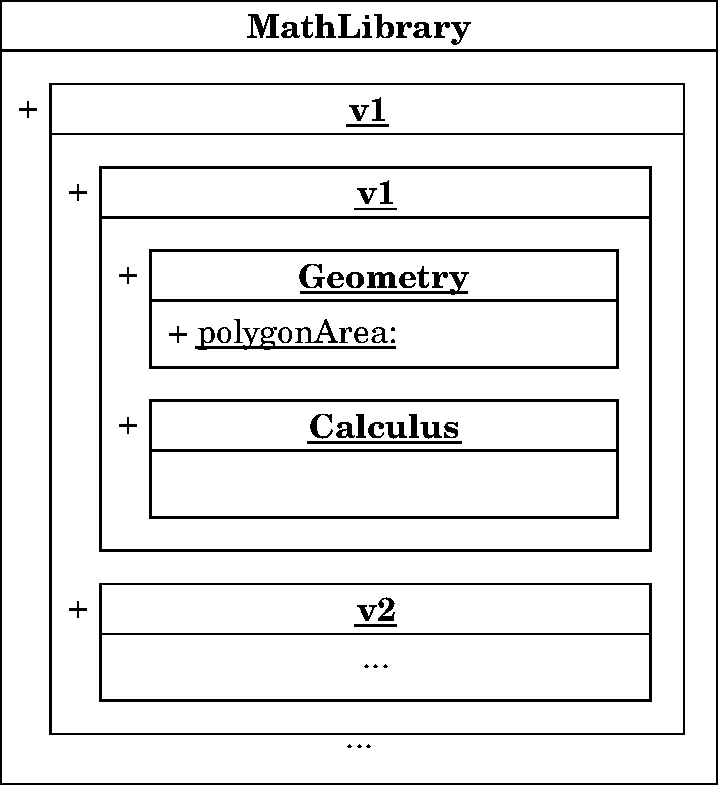
\includegraphics[width=0.5\textwidth]{usecase_define_version.pdf}
	\centering
	\caption{Module versioning}
	\label{fig:use_module_ver}
\end{wrapfigure}

Figure~\ref{fig:use_module_ver} shows how nested classes can be used for module versioning. In this example, we are developing a library for mathematical operations. The top-level class contains nested classes for every major version. Every major version can again have nested classes for minor versioning. In fact, this scheme can be used to have any kind of versioning system, as long as it is based in numbers.

Two versions of \texttt{MathLibrary} are installed in this example: version 1.1 and version 1.2. These versions can be referenced by writing \texttt{MathLibrary v1 v1} and \texttt{MathLibrary v1 v2}. Note, that even though all versions define classes with the same name, no class clashes occur. If a class in \texttt{MathLibrary} references another class in \texttt{MathLibrary}, the method lookup will look for classes in the same version of \texttt{MathLibrary}.

\subsection{Aliasing Module Versions}
Whenever an application requires a class from a library in a certain version, the application can either write down the fully qualified name of the class or create an alias. For example, the fully qualified name of the class \texttt{Calculus} in \texttt{MathLibrary} version 1.2 is \texttt{MathLibrary v1 v2 Calculus}. However, it is very likely that an application requires more than just one class from a library. In this case, an alias should be defined, because it keeps the required version number at a single point in the code (making it easy to change the version) and results in less verbose code.

\begin{figure}[!htp]
\begin{lstlisting}
<@\textbf{MyApplication>>MathLibrary}@>
    ^ Repository MathLibrary v1 v2

<@\textbf{MyApplication>>rectArea:}@> origin <@\textbf{extent:}@> extent
    ^ MathLibrary polygonArea: { 
        origin x @ origin y.
        (origin x + extent x) @ y.
        (origin x + extent x) @ (origin y + extent y).
        origin x @ (origin y + extent y) }
\end{lstlisting}
\caption{Defining class aliases}
\label{fig:use_alias}
\end{figure}

Figure~\ref{fig:use_alias} shows how class alias can be used to specify module versions at a single point in the code. The programmers defines a method\texttt{MathLibrary} returning the module in the required version. In \texttt{MyApplication>>rectArea:extent:}, the reference to \texttt{MathLibrary} will be replaced with \texttt{scope MathLibrary}, which will call the aliased method. Note, that in \texttt{MyApplication>>MathLibrary}, we have to reference the library with \texttt{Repository MathLibrary}, forcing the lookup to start at the root of our system. Otherwise, the method \texttt{MathLibrary} would call itself.

\paragraph{Helper Methods}
In Figure~\ref{fig:use_module_ver} the top-level class and major version should be a subclass of the class \texttt{Versioning}, a class provided by our system. This class contains convenience methods making it easier to work with version containers. The following list gives an overview of the helper methods \texttt{Versioning} provides.

\begin{itemize}
	\item \texttt{Versioning>>myLatest}: returns the latest version contained as a nested class in the receiver. For example, \texttt{MathLibrary myLatest} returns \texttt{MathLibrary v1}.
	\item \texttt{Versioning>>latest}: returns the lastest version in the receiver recursively. For example, \texttt{MathLibrary latest} returns \texttt{MathLibrary v1 v2}.
	\item \texttt{Versioning>>atLeast:}: returns the latest version recursively and asserts that its version number is greater than the parameter. For example, \texttt{MathLibrary atLeast: '1.1'} returns \texttt{MathLibrary v1 v2}, and \texttt{MathLibrary atLeast: '1.3'} throws an error.
\end{itemize}

\subsection{External Configuration}
Parameterized classes can not only be used to build mixins, but also externally configuarable modules. The basic idea is taken from Newspeak, where all module dependencies are encapsulated in a \texttt{platform} object. This platform object is installed along with the application source code and contains all libraries that the application depends on in the correct version~\cite{bracha2008newspeak}. This has the advantage that there is no need for a global namespace and all references to external classes are resolved using the platform object, effectively making import statements obsolete. A configurable module does not need to know anything about concrete implementations of external libraries, as long as the implementations provided in the platform implement the expected interfaces.

In our system, methods inside parameterized classes can reference arguments provided to the class accessor method. The idea is that, instead of referencing classes in the global namespace, the programmer references these arguments. The user of the module can then decide which exact implementation he wants to use.

\paragraph{Example}
Figure~\ref{fig:use_paintbrush} shows part of the implementation of simple drawing application. \texttt{PaintbrushWith:IO:} is a parameterized top-level class which takes as arguments a matrix implementation and a file IO library. The matrix implementation is used for storing the pixels inside the application. In the simplest case, this is could be the class \texttt{Matrix} from the Squeak standard library. It could, however, also be a class which stores pixels in a compressed form (e.g., using run-length encoding), but has \texttt{at:}, \texttt{at:put:}, \texttt{rows}, and \texttt{columns} as public API methods. \texttt{ReaderWriter} must be a class or object that supports reading and writing files on a pixel-by-pixel basis. Depending on which IO class the user of the library provides to \texttt{PaintbrushWith:IO:}, the application might for example generate JPEG files or PNG files.

\begin{figure}[!htp]
\begin{subfigure}[b]{\textwidth}
\centering
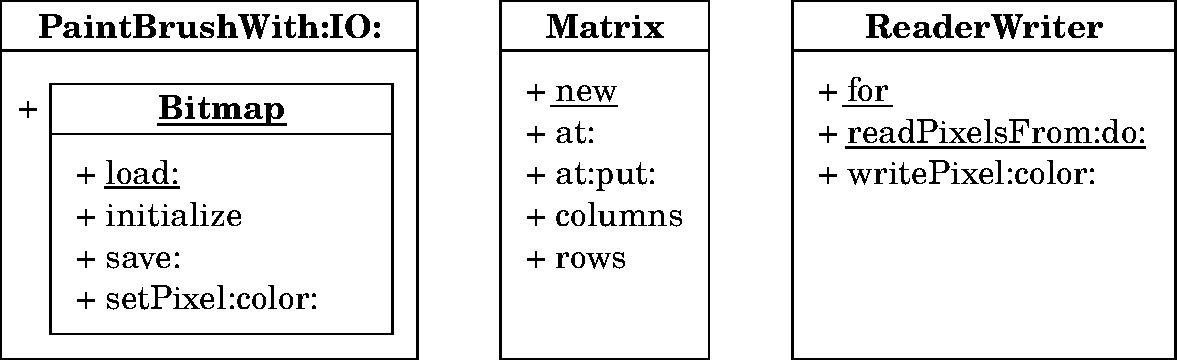
\includegraphics[width=0.8\textwidth]{usecase_paintbrush.pdf}
\caption{Overview of the \texttt{PaintBrushWith:IO:} module and dependent interfaces}
\end{subfigure}

\vspace{10pt}

\begin{subfigure}[b]{\textwidth}
\begin{lstlisting}
<@\textbf{PaintbrushWith:}@> Matrix <@\textbf{IO:}@> ReaderWriter
    <@\textcolor{OliveGreen}{\textbf{< class >}}@>
    ^ Object subclass

<@\textbf{(PaintbrushWith:}@> Matrix <@\textbf{IO:}@> ReaderWriter<@\textbf{) class>>Bitmap}@>
    <@\textcolor{OliveGreen}{\textbf{< class >}}@>
    ^ Object subclassWithInstVars: <@\textcolor{RoyalPurple}{'pixels'}@>

<@\textbf{(PaintbrushWith:}@> Matrix <@\textbf{IO:}@> ReaderWriter<@\textbf{) class>>Bitmap>>initialize}@>
    pixels := Matrix new.

<@\textbf{(PaintbrushWith:}@> Matrix <@\textbf{IO:}@> ReaderWriter<@\textbf{) class>>Bitmap>>}@>
        <@\textbf{setPixel:}@> aPoint <@\textbf{color:}@> aColor
    pixels at: aPoint put: aColor.

<@\textbf{(PaintbrushWith:}@> Matrix <@\textbf{IO:}@> ReaderWriter<@\textbf{) class>>Bitmap class>>}@>
        <@\textbf{load:}@> aFile
    <@\textcolor{Gray}{| instance |}@>
    <@\textcolor{Gray}{instance}@> := self new.
    ReaderWriter 
        readPixelsFrom: aFile
        do: [ :point :color | <@\textcolor{Gray}{instance}@> setPixel: point color: color ].
    ^ <@\textcolor{Gray}{instance}@>

<@\textbf{(PaintbrushWith:}@> Matrix <@\textbf{IO:}@> ReaderWriter<@\textbf{) class>>Bitmap>>save:}@> aFile
    <@\textcolor{Gray}{| writer |}@>
    <@\textcolor{Gray}{writer}@> := ReaderWriter BitmapWriter for: aFile.
    1 to: pixels columns do: [ :x |
        1 to: pixels rows do: [ :y | 
            <@\textcolor{Gray}{writer}@> writePixel: x@y color: (pixels at: x@y) ] ].
    <@\textcolor{Gray}{writer}@> close.
\end{lstlisting}
\caption{Source code for configurable application}
\end{subfigure}
\caption{Parameterized classes for external module configuration}
\label{fig:use_paintbrush}
\end{figure}

It is important to understand that the implementation of \texttt{PaintbrushWith:IO:} is entirely decoupled from the pixel data structure representation and the import/export functionality. It is up to the user of \texttt{PaintbrushWith:IO:} to configure the class as needed.

External configuration as shown in this example is similar to a constructor that accepts class objects as parameters and constructs and instance of the class with the class objects stored in instance variables. The difference to this approach is that, in our system, also class methods are bound to the passed arguments, because a new class object is constructed instead of an instance of a class. Furthermore, our system allows creating new nested classes with the argument as a superclass (mixins).

\section{Hierarchical Decomposition}
\label{sec:usecase_hierach_decomp}
One of the benefits of hierarchical decomposition is better readability and better understandability. Proper class nesting makes it easier for readers of the source code to understand which classes belong together and to find the class containing a certain functionality.

As an example, we took two simple computer games written in Squeak: SpaceCleanup\footnote{\url{https://github.com/matthias-springer/space-cleanup}}, a bomberman clone, and Breakout\footnote{\url{https://github.com/fniephaus/BroBreakout}} (Figure~\ref{fig:usecase_games}).

\begin{figure}[!htp]
\centering
\begin{subfigure}[b]{0.45\textwidth}
    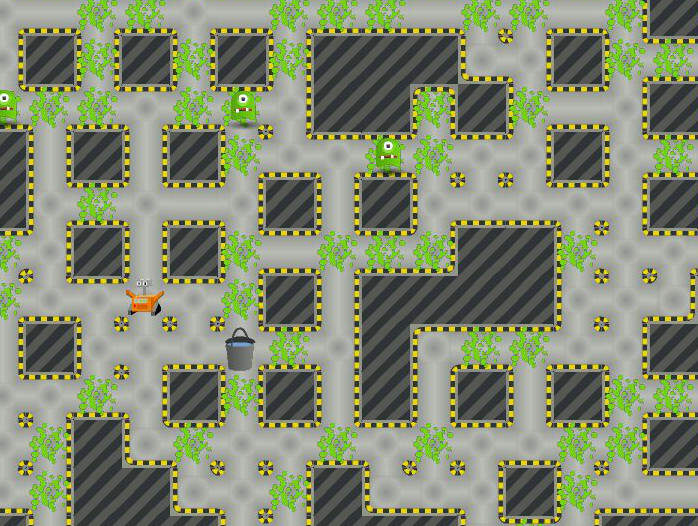
\includegraphics[width=\textwidth]{screen_scleanup.jpeg}
    \caption{SpaceCleanup}
\end{subfigure}
\qquad
\begin{subfigure}[b]{0.45\textwidth}
    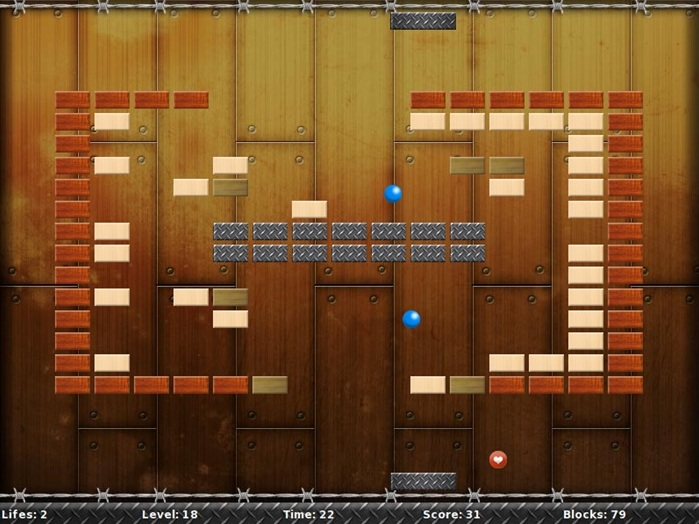
\includegraphics[width=\textwidth]{screen_breakout.jpeg}
    \caption{Breakout}
\end{subfigure}
\caption{Example games as subjects for hierarchical decomposition}
\label{fig:usecase_games}
\end{figure}

Figure~\ref{fig:usecase_sc_space} shows the original source code of SpaceCleanup and the source code after we introduced class nesting. The original source code already made use of packages, which can be compared to a single level of class nesting. The refactored source code is mostly unchanged, except for class name changes. What is interesting to see is that the class structure is already much more readable by just getting rid of all namespace prefixes. We can not only get rid of class prefixes, but also suffixes. For example, the \texttt{Builder}, \texttt{Item}, and \texttt{State} suffixes are omitted. It is now also possible to group classes together that belong together logically. For example, all both level builders are nested within \texttt{SpaceCleanup Level}. Similarly, all items are nested in \texttt{SpaceCleanup Level Items} (which is also a superclass of all items), which makes sense because a level consists of tiles and every tile can have items. An item cannot be used without a tile and a tile is never used outside a level. Note, that there exist two classes with the name \texttt{Random}, but they are nested in different classes.

\begin{figure}
\begin{subfigure}[b]{0.45\textwidth}
\dirtree{%
.1 \framebox{\textbf{SpaceCleanup}}. 
.2 EventDispatcher.
.2 Level.
.3 \textit{Builder}.
.4 GridPattern.
.4 Random.
.3 Tile.
.4 \textit{Item}.
.5 Bucket.
.5 \textit{Destructible}.
.5 Floor.
.5 Monster.
.6 \textit{Strategy}.
.7 MoveToPlayer.
.7 Random.
.5 \textit{Moving}.
.5 PickUp.
.5 Player.
.5 Portal.
.5 Slime.
.5 Wall.
.5 Water.
.2 \textit{State}.
.3 Building.
.3 Configuring.
.3 GameOver.
.3 GameWon.
.3 Paused.
.3 Running.
.2 Resources.
.2 UI.
.3 CheatWindow.
.3 ConfigurationWindow.
.3 Controls.
.3 GameInformation. 
}
\caption{Refactored project structure}
\end{subfigure}
\qquad
\begin{subfigure}[b]{0.45\textwidth}
\dirtree{%
.1 \framebox{\textbf{SpaceCleanup-Core}}.
.2 ScuEventDispatcher.
.2 ScuGame.
.2 ScuGameBuildState.
.2 ScuGameConfigState.
.2 ScuGameOverState.
.2 ScuGamePausedState.
.2 ScuGameRunningState.
.2 \textit{ScuGameState}.
.2 ScuGameWonState.
.2 \textit{ScuMonsterStrategy}.
.2 ScuMonsterRandomStrategy.
.2 ScuMonsterToPlayerStrategy.
}
\vspace{10pt}
\dirtree{%
.1 \framebox{\textbf{SpaceCleanup-Items}}.
.2 ScuBucket.
.2 \textit{ScuDestructibleItem}.
.2 ScuFloor.
.2 \textit{ScuItem}.
.2 ScuMonster.
.2 \textit{ScuMovingItem}.
.2 ScuPickUpItem.
.2 ScuPlayer.
.2 ScuPortal.
.2 ScuSlime.
.2 ScuWall.
.2 ScuWater.
}
\vspace{10pt}
\dirtree{%
.1 \framebox{\textbf{SpaceCleanup-Level}}.
.2 ScuLevel.
.2 \textit{ScuLevelBuilder}.
.2 ScuGridPatternLevelBuilder.
.2 ScuRandomLevelBuilder.
.2 ScuTile.
}
\vspace{10pt}
\dirtree{%
.1 \framebox{\textbf{SpaceCleanup-Resources}}.
.2 ScuResourceManager.
}
\vspace{10pt}
\dirtree{%
.1 \framebox{\textbf{SpaceCleanup-UI}}.
.2 ScuCheatWindow.
.2 ScuConfigurationWindow.
.2 ScuControls.
.2 ScuGameInformation.
}
\caption{Original project structure}
\label{fig:usecase_sc_origi_fig}
\end{subfigure}
\caption{SpaceCleanup game implementation with/without hierarchical decomposition}
\label{fig:usecase_sc_space}
\end{figure}

Figure~\ref{fig:usecase_breakout_game} shows the original source code of Breakout, as well as a refactored version. We did not change the source code, except for class names. All block-related classes are stored as nested classes in the class \texttt{Breakout Block}, which is also used to represent regular blocks in the game, that can be destroyed using \texttt{Racket}. \texttt{Breakout Block Boundary} represents a special block used for the design undestroyable borders of the game. All power ups are represented as classes and stored as nested classes in the abstract superclass \texttt{Breakout Powerup}. The structure of the refactored version is much clearer, because the original version did not take advantage of packages, probably due to the relatively small number of classes.

\begin{figure}[!htp]
\begin{subfigure}[b]{0.45\textwidth}
\dirtree{%
.1 \framebox{\textbf{Breakout}}.
.2 Level.
.3 Ball.
.3 Block.
.4 Boundary.
.4 Explosion.
.4 Racket.
.3 Builder.
.3 \textit{Powerup}.
.4 Accelerate.
.4 Ball.
.4 Decelerate.
.4 Enlarge.
.4 Shrink.
.3 World.
.2 \textit{View}.
.3 Level.
.3 Menu.
.3 Welcome.
.2 LevelStatistics.
.3 Item.
.2 MenuLabel.
}
\caption{Refactored project structure}
\end{subfigure}
\qquad
\begin{subfigure}[b]{0.45\textwidth}
\dirtree{%
.1 \framebox{\textbf{BroBreakout}}.
.2 BroBall.
.2 BroBlock.
.2 BroBoundary.
.2 BroBreakout.
.2 BroExplosion.
.2 BroLevelBuilder.
.2 BroLevelStatistics.
.2 BroLevelStatisticsItem.
.2 BroLevelView.
.2 BroLevelWorld.
.2 BroMenuLabel.
.2 BroMenuView.
.2 \textit{BroPowerup}.
.2 BroPowerupAccelerate.
.2 BroPowerupBall.
.2 BroPowerupDecelerate.
.2 BroPowerupEnlarge.
.2 BroPowerupShrink.
.2 BroRacket.
.2 \textit{BroView}.
.2 BroWelcomeView.
}
\caption{Original project structure}
\end{subfigure}
\caption{Breakout game implementation with/without hierarchical decomposition}
\label{fig:usecase_breakout_game}
\end{figure}

example: large project, where parts of the code can now be understood, given that we have hierarchical nesting. could be an example where grouping according to multiple criteria is needed (would result in n x m packages)

\section{Mixin Modularity with Parameterized Classes}
Parameterized classes can be used to build mixins. Mixins are not a special feature of this system: they are an application of our system and come for free by just having class nesting as described in the previous sections; they are an immediate consequence of parameterized classes. A mixin is a function that takes as an input a class and outputs a subclass with additional behavior, i.e., it is a class transformator. 

A mixin can be implemented by writing a class generator method with one parameter which is the input class. The method creates a subclass of that input class and returns it. Associated with that parameterized class generator methods is a set of instance-side methods and a set of class-side methods. These are the methods that will be added when applying the mixin.

\paragraph{Recursive Mixin Application}
A mixin can make sure another mixin is applied upon its application. This is done creating a subclass of a mixin application in the class generator method. Consequently, the system first creates a subclass of the base class, adds the methods of the inner mixin, then creates a subclass of the resulting class, and finally adds the methods of the outer mixin.

\paragraph{Example}
Figure~\ref{fig:concept_mixins} shows an example of parameterized classes and how they can be used to build mixins.

\begin{figure}[!htp]
    \centering
    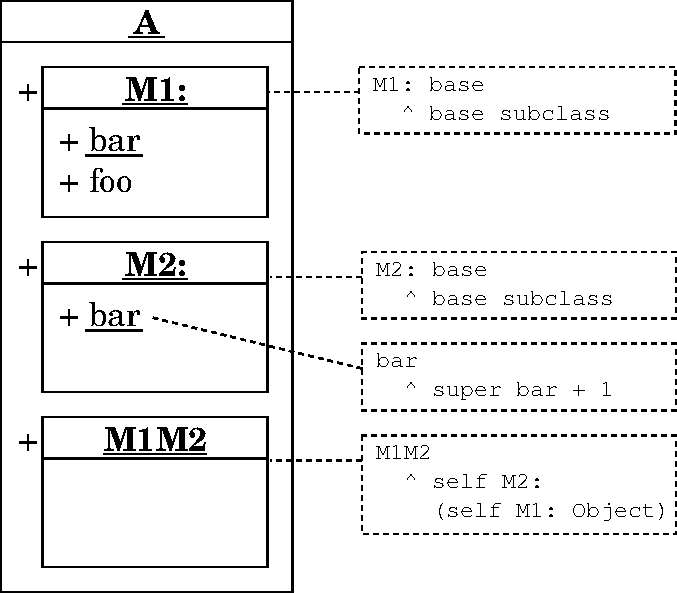
\includegraphics[scale=0.75]{nested_mixins.pdf}
    \caption{Implementation of Mixins with Nested Classes}
    \label{fig:concept_mixins}
\end{figure}

Two class generator methods \texttt{A M1:} and \texttt{A M2:} are defined, which take as input a base class and output a subclass with additional behavior. \texttt{A M1M2} is an application of both both mixins. \texttt{A M1M2}'s superclass is \emph{some} \texttt{A M2:}, whose superclass is \emph{some} \texttt{A M1:}, whose superclass is \texttt{Object}. Note, that \texttt{A M1:} and \texttt{A M2:} are not specific classes: we use this notation as a name for \emph{some} application of \texttt{A class>>M1:} and \texttt{A class>>M2:}, respectively. Therefore, even if two classes have the same name, they are not necessarily the same class if they names contain a colon.

Note, that evaluating \texttt{A M1: Object} multiple times returns different class object, since parameterized classes are not cached. However, \texttt{A M1M2} is cached, because it is a unary method. Therefore, calling \texttt{A M1M2} multiple times always returns the same class object.

The notation used in \texttt{A class>>M1M2} can be a bit confusing at first. That method first applies \texttt{A M1:} to \texttt{Object}, and then \texttt{A M2:}; however, in the source code, \texttt{A M2:} appears before \texttt{A M1:}. For readability reasons, and to support more features like pre-include hooks and post-include hooks, we present the Class Generator Pattern in Section~\ref{sec:usecase_classgen}.

\section{Unparameterized Class Generator Pattern}
\label{sec:usecase_classgen}
The syntax used for mixin application has a few shortcomings. For example, the statements \texttt{self A: (self B: Object))} means that mixin \texttt{B:} is applied to \texttt{Object}, and then mixin \texttt{A:} is applied to that result. The problem is that the source code statement does not reflect the order of mixin applications: the statement has to be interpreter from right to left. Another problem is that \texttt{A:} and \texttt{B:} are parameterized classes and parameterized classe cannot be referenced using an implicit \texttt{scope} receiver. Therefore, the programmer always has to write an explicit receiver.

Both problems can be solved by wrapping the mixin in an unparameterized class and adding a helper method to \texttt{Class}. We assume that name of the parameterized nested class is always \texttt{Mixin:}. Then, the helper method \texttt{<<} can be defined as shown in Figure~\ref{fig:usecase_class_lele}.

\begin{figure}[!htp]
\begin{lstlisting}
<@\textbf{Class>><< aMixin}@>
    ^ aMixin Mixin: self
\end{lstlisting}
\caption{Helper method on \texttt{Class} for unparameterized mixin wrapper classes}
\label{fig:usecase_class_lele}
\end{figure}

\paragraph{Example}
Figure~\ref{fig:usecase_unparam_class_gen} shows two mixins and a base class: \texttt{CollectionLogic} is a mixin that adds the methods \texttt{allSatisfy:} and \texttt{anySatisfy:}, and \texttt{CollectionFilter} is a mixin that adds the methods \texttt{detect:} and \texttt{select:}. All of these four methods can be implemented based on \texttt{do:}, which iterates through all elements of a collection. Consequently, these four methods are written in such a way, meaning that both mixins can be applied classes providing at lease this method.

\begin{figure}[!htp]
\begin{subfigure}[b]{\textwidth}
	\centering
	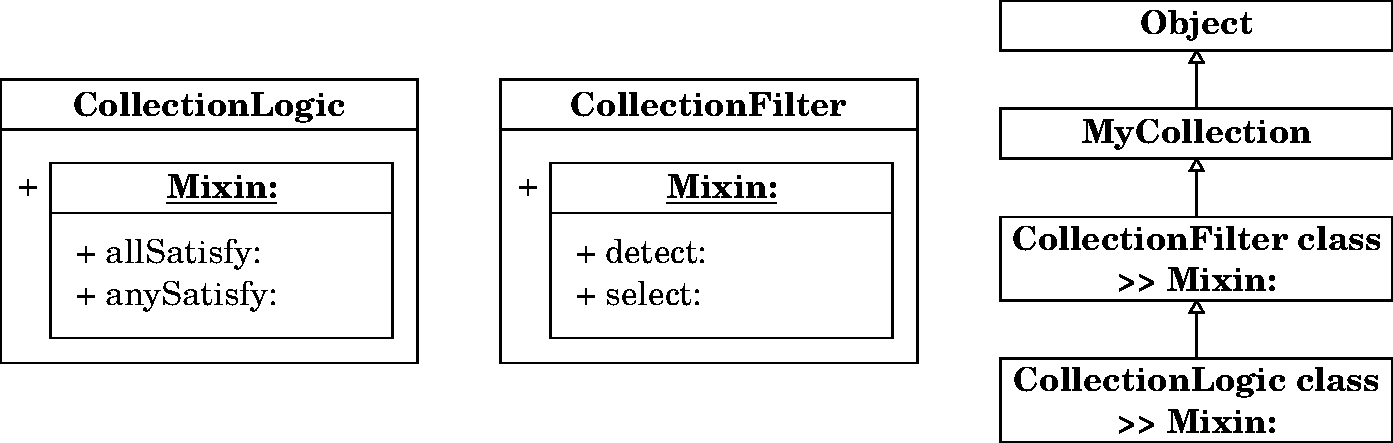
\includegraphics[width=0.95\textwidth]{usecase_classgen.pdf}
	\caption{Class diagram showing mixin and result of mixin application}
\end{subfigure}

\vspace{10pt}

\begin{subfigure}[b]{\textwidth}
\begin{lstlisting}
<@\textbf{CollectionLogic class>>Mixin:}@> base
    <@\textcolor{OliveGreen}{\textbf{< class >}}@>
    ^ base subclass

<@\textbf{(CollectionLogic class>>Mixin:}@> base<@\textbf{)>>allSatisfy:}@> aBlock
    self do: [ :each | 
        (aBlock value: each) ifFalse: [ ^ false ] ].
    ^ true

<@\textbf{(CollectionLogic class>>Mixin:}@> base<@\textbf{)>>anySatisfy:}@> aBlock
    self do: [ :each | 
        (aBlock value: each) ifTrue: [ ^ true ] ].
    ^ false

" (implementation of CollectionLogic omitted) "

<@\textbf{MyCollection>>do:}@> aBlock
    " Some implementation "

<@\textbf{FullCollection}@>
    <@\textcolor{OliveGreen}{\textbf{< class >}}@>
    ^ MyCollection << CollectionFilter << CollectionLogic
\end{lstlisting}
\caption{Definition and application of mixins}
\end{subfigure}
\caption{Unparameterized class generator pattern}
\label{fig:usecase_unparam_class_gen}
\end{figure}

\texttt{CollectionLogic} and \texttt{CollectionFilter} are wrappers around mixins, making it possible to access them like any unparameterized class. When a mixin is applied using the \texttt{<<} syntax, the receiver is sent to the \texttt{Mixin:} method. Therefore, the name of the actual mixin must always be \texttt{Mixin:}, as long as, \texttt{<<} is implemented as shown in Figure~\ref{fig:usecase_class_lele}. Note, that \texttt{<<} inverses the order of receiver and argument, which is why the statement in \texttt{FullCollection} can be read from left to right: first \texttt{CollectionFilter} and then \texttt{CollectionLogic} is applied to \texttt{MyCollection}.

\paragraph{Pre-Include Hooks and Post-Include Hooks}
The unparameterized class generator pattern allows the definition of pre-include hooks and post-include hooks. A pre-include hook is a method defined on the mixin wrapper, which is executed before the mixin was applied, with the base class as an argument. Similarly, a post-commit hook is executed after the mixin was applied, with the resulting class as an argument. 

Note, that the programmer can already write arbitrary code at the point where the mixin is applied. However, pre-include hooks and post-include hooks are provided by the mixin itself, and not by the user of a mixin.

\begin{figure}[!htp]
\centering
\begin{subfigure}[b]{0.45\textwidth}
\begin{lstlisting}
<@\textbf{Class>><< aMixin}@>
    <@\textcolor{Gray}{| result |}@>
    aMixin before: self.
    <@\textcolor{Gray}{result}@> := aMixin Mixin: self.
    aMixin after: <@\textcolor{Gray}{result}@>.
    ^ <@\textcolor{Gray}{result}@>
\end{lstlisting}
\caption{Mixin wrapper application}
\end{subfigure}
\qquad
\begin{subfigure}[b]{0.45\textwidth}
	\centering
	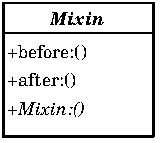
\includegraphics[scale=1]{abstract_mixin_classgen.pdf}
	\caption{Mixin wrapper base class}
\end{subfigure}
\caption{Implementation of pre-incude hooks and post-include hooks for mixins}
\label{fig:usecase_prepostincl}
\end{figure}

Figure~\ref{fig:usecase_prepostincl} shows how these hooks are implemented. Mixins with a pre-include hook or a post-include hook should be a subclass of the abstract class \texttt{Mixin}. This class provides empty \texttt{before:} and \texttt{after:} methods which should be overridden in subclasses and contain the pre-include hook or post-include hook.

In the previous paragraph, the unparameterized class generator pattern was presented as a tool to increase code readability. With regards to include hooks, this pattern is more: it is necessary to have some kind of wrapping. Include hooks shold not be defined on the mixin function itself, because all methods defined on the mixin function are added during mixin application. This is usually not desirable.

\section{Mixins as Composable Pieces of Behavior}
Mixins, as described in the last two sections, are class transformators. Given an existing class, they out a new subclass with additional or changed behavior. In Figure~\ref{fig:usecase_unparam_class_gen}, we started with \texttt{MyCollection}, a class containing only the \texttt{do:} method, and added additional behavior to it, resulting in the class \texttt{FullCollection}. 

Here is another point of view on the same situation: combine behavior from \texttt{CollectionFilter} and \texttt{CollectionLogic}, add an implementation of \texttt{do:}, and call it \texttt{FullCollection} (Figure~\ref{fig:mixin_composable}).

\begin{figure}[!htp]
\centering
\begin{subfigure}[b]{0.6\textwidth}
\begin{lstlisting}
<@\textbf{FullCollection}@>
    <@\textcolor{OliveGreen}{\textbf{< class >}}@>
    ^ (Object 
        << CollectionFilter 
        << CollectionLogic) subclass

<@\textbf{FullCollection>>do:}@> aBlock
    " Some implementation "
\end{lstlisting}
\end{subfigure}
\qquad
\begin{subfigure}[b]{0.25\textwidth}
    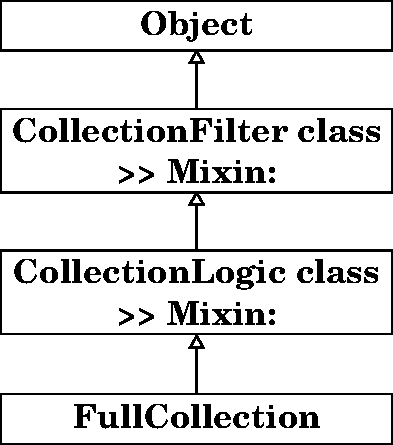
\includegraphics[width=\textwidth]{usecase_classgen_v2.pdf}
\end{subfigure}
\caption{Mixins as composable pieces of behavior}
\label{fig:mixin_composable}
\end{figure}

For readability reasons, our implementation provides a simplified notation that combines this kind of mixin application and subclassing (Figure~\ref{fig:usecase_subcl_mixin}). This new notation first applied mixins, and creates a subclass of the result afterwards. Note, that the notation reflects the order of subclassing: at first, \texttt{Mixin1} is applied, then \texttt{Mixin2}, then \texttt{Mixin3}, and finally a subclass is created with the additional methods defined on \texttt{NewClass}.

\begin{figure}[!htp]
\begin{subfigure}[b]{0.45\textwidth}
\begin{lstlisting}
<@\textbf{NewClass}@>
    <@\textcolor{OliveGreen}{\textbf{< class >}}@>
    ^ Object
        mixin: Mixin1
        mixin: Mixin2
        mixin: Mixin3
        subclassWithInstVars: <@\textcolor{RoyalPurple}{'foo bar'}@>
        classVars: <@\textcolor{RoyalPurple}{'Bar'}@>
        classInstVars: <@\textcolor{RoyalPurple}{'Foo'}@>
\end{lstlisting}
\caption{Mixin and subclass template}
\end{subfigure}
\qquad
\begin{subfigure}[b]{0.45\textwidth}
\begin{lstlisting}
<@\textbf{FullCollection}@>
    <@\textcolor{OliveGreen}{\textbf{< class >}}@>
    ^ Object
        mixin: CollectionFilter
        mixin: CollectionLogic
        subclassWithInstVars: <@\textcolor{RoyalPurple}{''}@>
\end{lstlisting}
\caption{Mixin and subclass example}
\end{subfigure}
\caption{Simplified notation for using subclassing and mixins}
\label{fig:usecase_subcl_mixin}
\end{figure}

The idea of mixins used as composable units of behavior is similar to traits~\cite{traitsschaerli}. However, there are some minor differences.
\begin{itemize}
    \item Mixins are not flat, but create an inheritance hierarchy. E.g., \texttt{FullCollection superclass} returns an application of \texttt{CollectionLogic class>>Mixin:} and not \texttt{Object}.
    \item No explicit conflict resolution is required. Traits raise an error whenever a method is added multiple times and the conflict is not resolved manually in the resulting class. The last applied mixin, on the other hand, overwrites predefined methods with the same name, but allows calling the original implementation using \texttt{super}.
\end{itemize}


\section{Traits}

\section{Extension Methods}
\label{sec:usecases_ext_meth}
There are cases, in which the functionality of an already class in a different module must be extended or changed. For example, this is the case when a bug in another library must be fixed. The programmer typically writes a method that replaces the existing one with the bug. Sometimes, extension methods are also used add additional behavior. For example, the \texttt{Morphic} package adds the convenience method \texttt{asStringMorph} to \texttt{String}. Sometimes it is sufficient to create a subclass of the class in question, and add the changed behavior only to the subclass. However, there are cases where the application code is not in control of instance creation.

An extension method can be added in our system by creating a nested classes whose class generator method returns an already existing class instead of a new subclass.

Consider, for example, that we want to add a method \texttt{asString} to the top-level class \texttt{CachedCollection} in Figure~\ref{fig:usecase_unparam_class_gen}. Figure~\ref{fig:use_ext_meth} shows how do define a method returning the string concatenation of all elements in the collection.

\begin{figure}[!htp]
\begin{lstlisting}
<@\textbf{MyApplication class>>FullCollection}@>
    <@\textcolor{OliveGreen}{\textbf{< class >}}@>
    ^ Repository FullCollection

<@\textbf{MyApplication class>>FullCollection>>asString}@>
    ^ String streamContents: [ :stream |
        self do: [ :each | stream nextPutAll: each asString ] ]
\end{lstlisting}
\caption{Extension methods using nested classes}
\label{fig:use_ext_meth}
\end{figure}

Note, that it is not possible to add extension methods to all parameterized classes or class specifications. Extension methods can only be added to concrete classes (i.e., class objects). For example, it is not possible, to add an extension method to all classes that are generated by \texttt{PaintBrushWith:IO:} in Figure~\ref{fig:use_paintbrush}; only a concrete class object (instantiation) can be extended.

Extension methods are dangerous because changes to existing methods could break other code relying on the old behavior. Numerous alternatives have been proposed, and we provide a brief overview of some of them in Section~\ref{sec:future_ext_meth}.

\chapter{Related Work}

\section{Class Name Clashes}

\subsection{Namespaces/Packages}
VisualWorks, Java, Ruby, Python

\subsection{Squeak Environments}

\subsection{Newspeak Modules}


\section{Dependency Management}

\subsection{Java Class Loader}

\subsection{Separate Compilation}

\subsection{External Configuration in Newspeak}


\section{Readability and Understandability}

\subsection{Smalltalk Packages}

\subsection{Hierarchical Decomposition}
Java, Python, Ruby, Newspeak, \ldots

\subsection{Information Hiding with Interfaces}


\section{Code Reuse}

\subsection{Multiple Inheritance}

\subsection{Mixins}
Ruby Modules, Python Multiple Inheritance, Newspeak, Jigsaw

\subsection{Traits}
Squeak implementation

\chapter{Future Work}
\label{sec:future}
In this section, we give an overview of possible areas of future work. We also point of deficiencies of \msname that we want to address in future versions.

\section{Classes as Instance-side Members}
\label{sec:future_inst_side}
Java and Newspeak support nested classes as instance-side members (non-static member classes). Earlier versions \msname included support for instance-side nested classes, but this caused difficulties in the implementation. 

\begin{itemize}
	\item \emph{Method lookup:} Classes can now be enclosed in instances instead of classes. We are not sure whether a message send to \texttt{enclosing}, \texttt{outer}, or \texttt{scope} should also lookup methods on the class side whenever a message was not understood on the instance side. It would certainly be good style to nest classes that do not need access to instance-specific state as class class-side members. These classes should then be accessible within an instance using an implicit receiver send or the \texttt{scope} keyword.
	\item \emph{\texttt{outer}/\texttt{enclosing} cannot be early bound:} These keyword might have to start their lookup in an instance. Therefore, these keywords cannot be bound as literals, which are stored in methods and, therefore, shared among all instances.
	\item \emph{Possible memory issues:} In contrast to Java, \msname would generate a new class every time an instance-side member class is accessed. This could lead to memory and performance issues.
\end{itemize}

In addition to these difficulties, we are currently unclear about what the exact benefits of instance-side nested classes are. They can be used to build mixins, but the we achieve the same functionality with parameterized classes (see Section~\ref{sec:rel_mixins1}). In Java, non-static member classes are used to implement interface adapters that need access to the enclosing instance~\cite{Bloch:2008:EJ:1377533} (see Section~\ref{sec:rel_ns_pkg_cls_nesting}). This is, however, the only pattern for non-static member classes we could find in literature, and the same functionality can be achieved by implementing the adapter as a class-side nested class with an instance variable holding a reference to the adaptee.

As a consequence, we removed support for instance-side nested classes, but we might add it again at a later point of time, if it needed.

\section{Bytecode Transformation}
Whenever a nested class specification is instantiated in \msname, all methods in the specification are complied in the target class. When using parameterized classes, this process happens multiple times, once for every target class. However, the bytecode is almost the same for every target class and differs only for reads/writes to instance variables (see Section~\ref{sec:impl_ch_inst_cl_vars}). In addition, \texttt{enclosing} and \texttt{outer} must be bound to different literals.

This process could be optimized by caching compiled methods and replacing affected bytecodes and literals during instantiation. For example, instead of recompiling the entire method, all references to instance variables could be replaced with bytecodes with the correct indices in a linear pass through the compiled method.

In Newspeak, slots (instance variables) cannot be accessed directly. They are always accessed through automatically-generated accessor methods. Therefore, all references to slots are message sends. Consequently, the bytecode of a method for two different instantiations is always the same.

\section{Squeak Integration}
As of now, the integration of \msname in Squeak is still limited. For example, the new class browser does not have any refactoring tools yet. Furthermore, all Squeak classes should be migrated to classes in \msname, eventually, making \texttt{Repository} (a separate \texttt{globals} dictionary for \msname) obsolete. As described in Section~\ref{sec:impl_module_rep}, a single top-level class \texttt{Smalltalk} should contain all modules and Squeak base classes. Restructuring Squeak base classes in a hierarchical way will probably be the biggest and most tedious task. 

The Newspeak class organization might be a good starting point. Black et al. described how traits can be used to modularize Smalltalk collection classes~\cite{Black:2003:ATS:949305.949311}, which might be another good starting point for restructuring these classes.

\section{Extension Methods}
\label{sec:future_ext_meth}
In Smalltalk, an extension method is a method that extends an already existing class in another package. Additional methods can be defined on the instance side and and on the class side. Adding new instance/class variables or removing methods is not supported. In \msname, extension methods can be written by defining a class extension: a nested class with a class generator method that returns an already existing class.

Extension methods in Smalltalk and in \msname are controversial because they do not have proper conflict handling. If an extension method is defined and the target class has already a method with the same name, the original method is replaced, possibly breaking other code. Extension methods can be used to add new functionality to existing classes required by libraries (e.g., methods for the visitor design pattern). If two libraries add extension methods with the same name, the second extension always wins. In addition, removing an extension method does not restore the previous state: the original method has to be restored manually by the programmer.

Smalltalk extension methods break modularity. It is not possible to compose two modules providing colliding extension methods, because there is currently no way to resolve method conflicts without changing the source code of at least one of the modules. Furthermore, modules providing extension methods are not easily replacable, because the original state is not restored once a module is removed from the system.

Other programming languages (e.g., Ruby) have a concept similar to extension methods in Smalltalk. A variety of alternatives to extension methods have been proposed. In the rest of this chapter, we give a brief overview of some of them. Future versions of \msname might incorporate one of these alternatives.

\paragraph{Classboxes}
A classbox is a container of classes and methods. Classes can either be defined or imported into a classbox (from another classbox). Within a classbox, additional methods can be added or replaced on imported classes (\emph{local rebinding}). Code executed in the context of certain classbox has a modified method lookup: the system tries to lookup methods defined in the classbox first, and then proceeds with the ordinary method lookup (receiver class and superclass hierarchy)~\cite{bergel:inria-00533446}.

A classbox effectively acts as a sort of sandbox. Every classbox can define its own extensions methods for imported classes. Duplicate extension methods are not a problem as long as they are defined in different classboxes. 

Implementations of classboxes exist for Squeak~\cite{bergel:inria-00533446} and Java. Classbox/J is a Java implementation which does not only allow redefining fields and methods but also member classes (nested/inner classes)~\cite{Bergel:2005:CCS:1094811.1094826}.

\paragraph{Ruby Refinements}
In Ruby, all classes and modules are open for extensions. At any position in the program, existing classes can be modified, possibly breaking other code. Refinements are a way to confine class/module extensions to certain classes. A refinement can be defined as part of a module. Whenever the module is included, the refinement is active for code written in the including class~\cite{Carlson:2015:RC:1212915}. Other code is not affected.

\paragraph{Context-oriented Programming}
Context-oriented programming (COP) is a mechanism to modularize heterogeneous crosscutting concerns~\cite{Hirschfeld08context-orientedprogramming}. In layer-based context oriented programming, crosscutting concerns are grouped in layers. A layer is a set of partial method definitions (possibly from different classes). Every partial method definition belongs to exactly one base method. Whenever a layer is active, the system executes the partial methods defined in the layer instead of the corresponding base methods. Multiple layers can be active at the same time, effectively building a layer composition stack. A partial method can contain a \texttt{proceed} statement, which will call the next partial method, i.e., the partial method defined in the next layer on the layer composition stack. If there is no next layer defining a partial method for the corresponding base method, the system will call the base method.

Every module could group its extension methods in a separate layer, activate that layer whenever code from the module is run, and deactivate the layer afterwards. Most COP implementations support scoped layer activation~\cite{Appeltauer:2009:CCP:1562112.1562118}, which essentially activates a layer, then runs a method or function/block closure, and then deactivates the layer again.

With context-oriented programming, duplicate extension methods are no longer a problem, as long as they are contained in different layers as partial method definitions.

%\paragraph{Worlds}
%better way is needed (e.g., class boxes, refinements, COP, world (paper viewpoints), monkey patching). return already existing class in generator method

\section{Extending Inherited Nested Classes without Subclassing}
The way inherited nested classes can be extended without subclassing has two deficiencies. Firstly, there is currently no notation to add new instance variables to the extended class, because the subclass statement is part of the corresponding method in the superclass. Secondly, nested classes of already extended classes cannot be further extended, because a \texttt{super} call would not call the original class accessor method. Instead, the method lookup would start in the superclass of extended class (which is the same class as the not yet extended class).

It is still unclear, if extending inherited nested classes without subclassing should be forbidden in favor of the variant \emph{with subclassing}. Other programming languages like Jx do this by default~\cite{Nystrom:2004:SEV:1028976.1028986}. Extending inherited nested classes with subclassing would solve the problems described above and is already possible. However, forbidding \emph{extending without subclassing} is difficult without restricting the ability to write extension methods, which is technically a very similar concept.

\section{Dependency Management}
Nested classes in \msname can be used to store modules in different versions. There is at the moment no convenient way to share modules with other developers, except for exporting the module and importing it again. Future versions of \msname might have a central remote repository from which modules are automatically downloaded (similar to a Maven repository) if a module is referenced that is available in the image. The corresponding functionality could be part of a \texttt{doesNotUnderstand:} handler in \texttt{Repository}, which is the data structure holding references to all modules installed in the image.

There are also ideas for a better integration of the underlying source code management system (e.g., git) in \msname. If \msname is aware of commits, it can not only be used to run applications in certain versions, but also to run applications at a certain commit. Whether the source code management system should be completely reimplemented in \msname or be external and under control of \msname is still open to discussion.

\section{Language-supported Version Control}
In \msname, different versions of the same module are represented as different nested classes. The same mechanism could be used to integrate revision-based version control systems in Squeak/Smalltalk~\cite{springerniephaus}. Every revision/commit would then be represented by a separate nested class. \msname would ensure that nested classes are created automatically based on the revisions in the underlying version control system. Version control operations (e.g., commits and merges) could be invoked by sending messages to a nested class representing a revision.

\begin{figure}[!htp]
	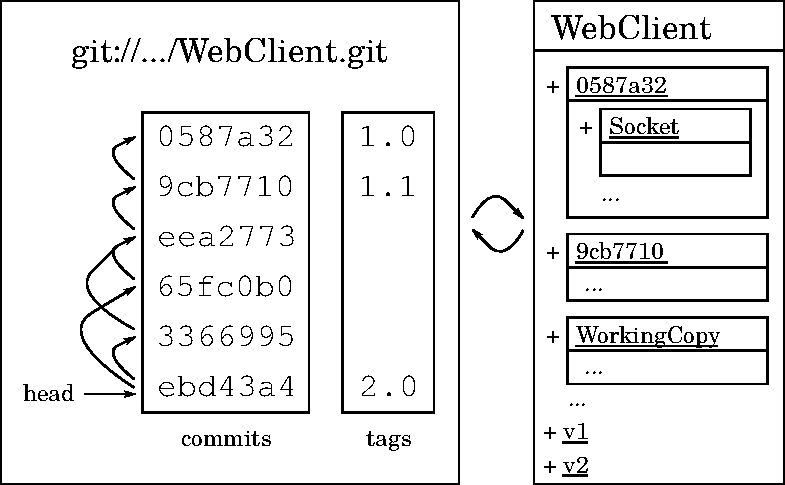
\includegraphics[width=0.75\textwidth]{matriona_concept.pdf}
	\centering
	\caption[Example: git-based version control with nested classes.]{Example: git-based version control with nested classes. \texttt{WebClient} is a module and every commit in the underlying version control system corresponds to an automatically-generated nested class in \msname.}
	\label{fig:fut_vers_control_git}
\end{figure}

Figure~\ref{fig:fut_vers_control_git} shows an example of a module named \texttt{WebClient}. The source code is stored in a git repository. Every commit in git corresponds to a nested class whose name is the SHA-1 hash of the commit. \msname takes care of the synchronization between the repository and the nested classes in the Squeak image. The programmer would always modify the source code in the class \texttt{WorkingCopy} and send a message like \texttt{commit:} to this class in order to perform a commit in the git repository. git tags could be used to provide a versioning scheme that is mirrored in the version control system.

This mechansim would allow the programmer to access any revision in the Squeak image without having to load the source code for a certain revision manually. Furthermore, multiple revisions of the same module could be run at the same time. Having version control in the Squeak image would also reduce the number of tools involved in the software development process and get rid of the conceptual break of leaving the image for committing to a git repository (see Section~\ref{sec:impl_scm_chap}).
% automatically download dependencies
% generate list of all dependencies
\chapter{Summary}
comparison with Newspeak: many ideas taken from it, but too complex

%\blinddocument

\printbibliography
\clearpage
\appendix
%% ggf:
% \part{Appendix}
% \label{part:appendix}

\chapter{Implementation Details}

\section{Determining the Lexical Scope}
\label{sec:app_lexical_scope}

\begin{figure}[!htp]
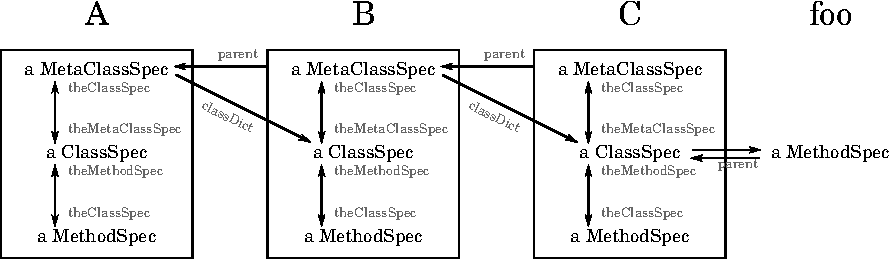
\includegraphics[width=\textwidth]{lexical_scope_app_ex.pdf}
\caption[Example: Detailed meta model]{Example: Detailed meta model.}
\end{figure}

\begin{figure}[!htp]
\begin{lstlisting}
MethodSpecification>>lexicalScopeIn: cls
    | enclosingClasses currentCls currentMetaClassSpec |
    enclosingClasses := OrderedCollection new.
    currentCls := cls.
    currentMetaClassSpec := self parent parent.

    enclosingClasses add: (currentCls := 
        (currentMetaClassSpec theClassSpec theMethodSpec 
            instantiations at: currentCls) first).

    [ currentMetaClassSpec parent isNil ] whileFalse: [
        currentMetaClassSpec := currentMetaClassSpec parent.
        enclosingClasses add: (currentCls := 
            (currentMetaClassSpec theClassSpec theMethodSpec 
                instantiations at: currentCls) first) ].

    ^ enclosingClasses
\end{lstlisting}
\caption[Determining the lexical scope of a method]{Determining all enclosing classes in the lexical scope of a method.}
\end{figure}

\section{Traits}
\label{sec:app_traits}

%%% Local Variables: 
%%% mode: latex
%%% End: 

\backmatter
\markboth{}\relax

% BAMA-O (2009) §24.8
%  Am Schluss der Arbeit hat die/der Kandidat/in  zu versichern, dass 
%  sie/er sie selbstständig verfasst sowie keine anderen Quellen und 
%  Hilfsmittel als die angegebenen benutzt hat.
% BAMA-O (2013) §30.6
%  Am Schluss der Arbeit hat die Kandidatin bzw. der Kandidat zu versichern,
%  dass sie bzw. er die Arbeit selbstständig verfasst und keine anderen
%  Quellen und Hilfsmittel als die angegebenen benutzt hat.
\defaultstatement
\end{document}
%%% Local Variables:
%%% mode: latex
%%% TeX-master: t
%%% End:
